\documentclass[a4paper,12pt]{article}

% Packages
\usepackage[utf8]{inputenc}
\usepackage[T1]{fontenc}
\usepackage{times}
\usepackage[top=1.2in,bottom=1in,left=1in,right=1in,headheight=28pt,headsep=14pt]{geometry}
\usepackage{graphicx}

\usepackage{float} % for figure placement specifier [H]
\usepackage{enumitem}
\usepackage{longtable}
\usepackage{array}
\usepackage{booktabs}
\usepackage{fancyhdr}
\usepackage{titlesec}
\usepackage{setspace}
\usepackage{parskip}
\usepackage{amssymb}
\usepackage[titles]{tocloft}
\usepackage{hyperref}

% ---- Header/Footer setup (matching Word: two-line header, no rule) ----
\pagestyle{fancy}
\fancyhf{}
\fancyhead[L]{\parbox[b]{\textwidth}{\footnotesize\textbf{\textit{Software Requirements Specification for Design and Implementation of a Mentor Caring System}}\\[2pt]\mbox{}\hfill\textbf{\textit{Page \thepage}}}}
\renewcommand{\headrulewidth}{0pt}
\renewcommand{\footrulewidth}{0pt}

% ---- Section heading formatting (matching Word style) ----
% Section: e.g. "1. Introduction" 18pt bold
\titleformat{\section}{\normalfont\fontsize{18}{22}\bfseries}{\thesection.\quad}{0pt}{}
\titlespacing*{\section}{0pt}{24pt}{12pt}
% Subsection: e.g. "1.1 Purpose" 14pt bold
\titleformat{\subsection}{\normalfont\fontsize{14}{17}\bfseries}{\thesubsection\quad}{0pt}{}
\titlespacing*{\subsection}{0pt}{18pt}{8pt}
% Subsubsection: e.g. "3.1.1 Description and Priority" 12pt bold
\titleformat{\subsubsection}{\normalfont\fontsize{12}{15}\bfseries}{\thesubsubsection\quad}{0pt}{}
\titlespacing*{\subsubsection}{0pt}{12pt}{6pt}

% ---- TOC formatting (matching Word: bold for sections, indentation for subsections) ----
\renewcommand{\cftsecfont}{\bfseries}
\renewcommand{\cftsecpagefont}{\bfseries}
\setlength{\cftsubsecindent}{2em}
\setlength{\cftsubsubsecindent}{4em}
\renewcommand{\cftsecleader}{\cftdotfill{\cftdotsep}}

% Body text: 12pt, single spacing (matching Word)
\setstretch{1.15}

% Graphics path
\graphicspath{{images/}{ver1.2_transitionDiagram/}{ver1.3_Sequence diagrams and class diagrams/}}


% Hyperref setup
\hypersetup{
    colorlinks=true,
    linkcolor=black,
    urlcolor=blue,
    citecolor=black
}

\begin{document}

%--------------------------------------------------------------
% Title Page (matching Word layout: thick top rule, left-aligned title, right-aligned metadata)
%--------------------------------------------------------------
\begin{titlepage}
\thispagestyle{empty}
\vspace*{0.5cm}

% Thick horizontal rule at top
\noindent\rule{\textwidth}{3pt}

\vspace{1.5cm}

% Title block left aligned, large bold
{\fontsize{26}{31}\selectfont\bfseries\raggedright
Software Requirements Specification\par}

\vspace{0.8cm}

{\fontsize{14}{17}\selectfont\bfseries\raggedright
for\par}

\vspace{0.8cm}

{\fontsize{26}{31}\selectfont\bfseries\raggedright
Design and Implementation of a Mentor Caring System\par}

\vfill

% Right-aligned metadata block
\begin{flushright}
{\fontsize{12}{15}\selectfont\bfseries
Version 1.3 \textit{approved}\\[1cm]
Prepared by\\
Wang Zhengyang 2330031281 FULL\\
Zhang Yaling 2330026222 FULL\\
Chen Zhengyang 2330024028 FULL\\
Liu Boyu 2330016025 FULL\\
Li Jinshang 2230026075 FULL\\
Wang Weihang 2230026157 FULL\\[0.8cm]
Group B04\\[0.5cm]
2026/4/4
}
\end{flushright}

\vspace{1cm}
\end{titlepage}

%--------------------------------------------------------------
% Table of Contents
%--------------------------------------------------------------
\newpage
\thispagestyle{fancy}
\setcounter{page}{2}
\renewcommand{\thepage}{\roman{page}}

% "Table of Contents" heading matching Word style
\renewcommand{\contentsname}{\fontsize{18}{22}\selectfont\bfseries Table of Contents}
\tableofcontents

\vspace{1cm}

%--------------------------------------------------------------
% Revision History
%--------------------------------------------------------------
% Revision History
\section*{Revision History}
\addcontentsline{toc}{section}{Revision History}

\begin{longtable}{|p{3.5cm}|p{2cm}|p{6cm}|p{2cm}|}
\hline
\textbf{Name} & \textbf{Date} & \textbf{Reason For Changes} & \textbf{Version} \\
\hline
Li Jinshang,\newline
Zhang Yaling,\newline
Liu Boyu,\newline
Wang Zhengyang,\newline
Chen Zhengyang
&
2026-03-12
&
Basic SRS file implementation\newline
Context model and Use case diagram first design
&
1.0 \\
\hline
Li Jinshang,\newline
Zhang Yaling,\newline
Liu Boyu,\newline
Wang Zhengyang,\newline
Chen Zhengyang\newline
Wang Weihang
&
2026-03-19
&
Section 3 Use Case updated\newline
Section 4 UI Reference released\newline
Section 5 old problems fixed
&
1.1 \\
\hline
Liu Boyu,\newline
Li Jinshang,\newline
Zhang Yaling,\newline
Wang Zhengyang,\newline
Chen Zhengyang\newline
Wang Weihang
&
2026-03-28
&
State transition diagrams created for all use cases\newline
UI diagrams created for all use cases\newline
Basic scenarios created for all use cases
&
1.2 \\
\hline
Liu Boyu,\newline
Li Jinshang,\newline
Zhang Yaling,\newline
Wang Zhengyang,\newline
Chen Zhengyang\newline
Wang Weihang
&
2026-04-04
&
Appendix B Sequence Diagram updated\newline
Appendix B Class Diagram updated\newline
ID mappings for the UI and other diagrams fixed
&
1.3 \\
\hline
\end{longtable}

%--------------------------------------------------------------
% Switch to Arabic page numbering
%--------------------------------------------------------------
\clearpage
\setcounter{page}{1}
\renewcommand{\thepage}{\arabic{page}}

%--------------------------------------------------------------
% 1. Introduction
%--------------------------------------------------------------
% Section 1: Introduction
\section{Introduction}

\subsection{Purpose}

This document specifies the software requirements for the Mentor Caring System (MCS) V1.0 developed for the BNBU Mentor Caring Programme. It fully covers all core functional and non-functional requirements of the MCS, including the functional permissions of all role users, data interaction rules, system operation processes and basic interface requirements. This SRS is a complete specification for the entire MCS system and does not involve only a part or a single subsystem of the overall system, serving as the fundamental basis for the subsequent design, development, testing, and acceptance of the MCS.

\subsection{Document Conventions}

\begin{enumerate}
\item \textbf{Font and Highlighting Conventions:} Key system roles (e.g., \textbf{Administrator}, \textbf{Faculty Consultant}), core functions (e.g., \textbf{Allocate Mentors}, \textbf{Generate Summary Report}) and special terms (e.g., \textbf{Mentor Caring System}, \textbf{MCS}) are marked in bold for emphasis; file formats (e.g., \textit{Excel}, \textit{Word}) and data fields (e.g., \textit{Student ID}, \textit{Group ID}) are marked in italic.

\item \textbf{Requirement Priority Inheritance:} The priority of detailed functional requirements is inherited from the higher-level module requirements where they are located. The overall requirements of the MCS are divided into three priority levels: High (core and indispensable functions for the operation of the Mentor Caring Programme), Medium (auxiliary functional requirements for improving system usability), and Low (optimization requirements for functional experience, implementable in follow-up versions). If an individual detailed requirement has a different priority from its higher-level module, it will be marked independently in the corresponding section.

\item \textbf{Numbering Conventions:} The document adopts a hierarchical numbering system (e.g., 1, 1.1, 1.1.1) for chapters, sections and specific requirements; functional goal serial numbers use Arabic numerals with parentheses (e.g., 1), and operational step serial numbers use lowercase Arabic numerals with periods (e.g., 1.).

\item \textbf{Nomenclature Conventions:} The full name \textbf{Mentor Caring System} is used for the first mention in each chapter, followed by the abbreviation \textbf{MCS} for subsequent references; all role and function names are consistent with the definitions in the BNBU Mentor Caring Programme official description.
\end{enumerate}

\subsection{Intended Audience and Reading Suggestions}

This document is intended for multiple stakeholders involved in the Mentor Caring System (MCS), including software developers, project managers, system testers, BNBU end users (administrators, faculty consultants, mentors, etc.), system maintainers and documentation writers.

The remainder of this SRS is organized in a logical, hierarchical structure from overall system overview to detailed technical requirements. Chapter 2 presents the overall description of the product, including its perspective, core features, user classes, operating environment and key assumptions. Chapter 3 details the specific system features that realize the product's core functions. Chapter 4 specifies all external interface requirements, covering user, hardware, software and communications interfaces. Chapter 5 outlines nonfunctional requirements such as performance, safety, security and software quality attributes. Chapter 6 lists other supplementary requirements, and the appendices provide a glossary, analysis models and an issues list for reference.

For a structured reading experience, all readers are recommended to start with Chapter 1 (Introduction) to grasp the basic background, purpose and scope of the MCS. End users may then focus on Chapter 2 (Overall Description) to understand the system's core features and role-based functions, and may skip the technical details in subsequent chapters. Developers and testers should read the full document in sequence, with key focus on Chapter 3 (System Features), Chapter 4 (External Interface Requirements) and Chapter 5 (Nonfunctional Requirements) to guide system design, development and testing. Project managers should prioritize Chapter 1, Chapter 2 and the priority of requirements across the document to plan project progress and resource allocation. Documentation writers and system maintainers should review the entire SRS, with additional attention to the appendices and detailed functional specifications to compile user manuals and support post-launch system maintenance.

\subsection{Project Scope}

The Mentor Caring System (MCS) is a dedicated supporting management system for BNBU's Mentor Caring Programme, which digitizes the programme's management by realizing mentor allocation, interview record reporting, appointment arrangement, summary report generation and information tracking, and interfaces with the existing school database to assign differentiated permissions for all relevant roles, aligning with BNBU's goal of improving the informatization level of student management work.

\subsection{References}

\begin{enumerate}
\item project description MCS long version [SE\_SDW\_Project Long Description 2025-2026-2 V.1.0]
\end{enumerate}

%--------------------------------------------------------------
% 2. Overall Description
%--------------------------------------------------------------
% Section 2: Overall Description
\section{Overall Description}

\subsection{Product Perspective}

The Mentor Caring System (MCS) is a new, self-contained software product developed exclusively for the BNBU Mentor Caring Programme, which aims to digitalize and standardize the management of the programme's daily operations and related activities for all undergraduate students of BNBU. This system is an independent supporting management tool and not a follow-on product of any existing software series, nor a replacement for other school information systems.

MCS interfaces with the existing BNBU school database (which stores staff and students' accounts, passwords, names and role attributes) to realize unified user identity authentication. It does not act as a component of a larger system, and all core functions (e.g., mentor allocation, interview record management, appointment arrangement) are built within the independent MCS framework. The system only interacts with the BNBU school database for data reading and verification during user login, without modifying or managing the original data of the school database.

\begin{figure}[htbp]
\centering
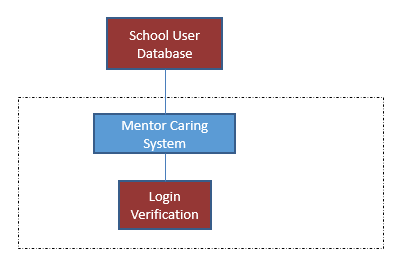
\includegraphics[width=0.5\textwidth]{context_model.png}
\caption{Context model of the Mentor Caring System}
\label{fig:main-context-model}
\end{figure}

\subsection{Product Features}

MCS is built around the core goals of the BNBU Mentor Caring Programme, providing role-based differentiated functional modules to realize the full-process digital management of the programme. The high-level core features are summarized as follows, with detailed specifications in Section 3:

\begin{sloppypar}
\begin{enumerate}
\item \textbf{Role Management \& Permission Allocation:} Supports hierarchical permission setting for six user roles, realizes unified identity authentication via the BNBU school database, and allows flexible configuration of the school's faculty-department-major organizational architecture (manual/Excel import).

\item \textbf{Mentor \& Student Allocation Management:} Facilitates batch import of mentor-student allocation information via Excel, supports manual adjustment of group mentors and group student members, and retains all historical information of students during any adjustment operation.

\item \textbf{Information Query \& Statistics:} Provides multi-dimensional search functions for student, mentor and system log information (supporting precise and conditional screening), and enables batch export of specified information to Word files based on academic year, department, mentor and student name.

\item \textbf{Interview Management:} Supports mentors to add, modify and delete interview records of their supervised students, and allows batch export of interview records to Word files for statistical and archival purposes.

\item \textbf{Online Communication \& Appointment:} Realizes two-way text communication between different roles, and supports the mentor-student interview appointment function (including mentor-set available time slots, venue confirmation and email notification for both parties).

\item \textbf{Special Case Processing:} Establishes a tiered forwarding mechanism for student special cases, from mentors to MCP coordinators and then to faculty consultants, to ensure timely follow-up of key student issues.

\item \textbf{System Log Monitoring:} Records the login/logout time and core function usage of all users, and provides log query and viewing permissions for designated roles to track system operation status.
\end{enumerate}
\end{sloppypar}

The Mentor Caring System (MCS) provides a centralized digital platform to support the BNBU Mentor Caring Programme. The system organizes its major functions into several groups of related capabilities.

First, the system supports role-based access control and identity authentication through the BNBU school database, ensuring that administrators, faculty consultants, mentors, students, MCP coordinators and supporting staff can access functions according to their permissions.

Second, the system manages mentor--student allocation and organizational structures, allowing faculty consultants to import or modify information about faculties, departments, majors, mentoring groups and student membership through Excel templates or manual operations.

Third, the system provides information management and query services, enabling users to search student records, mentor information and system logs, and export selected records into Word documents for reporting and archiving.

Fourth, the system supports interview record management and appointment scheduling between mentors and students. Mentors can create, modify or delete interview records and arrange available appointment time slots for students.

Finally, the system enables internal communication among different user roles through text messages and notifications, including forwarding special student cases from mentors to MCP coordinators and faculty consultants for further follow-up.

\begin{figure}[htbp]
\centering
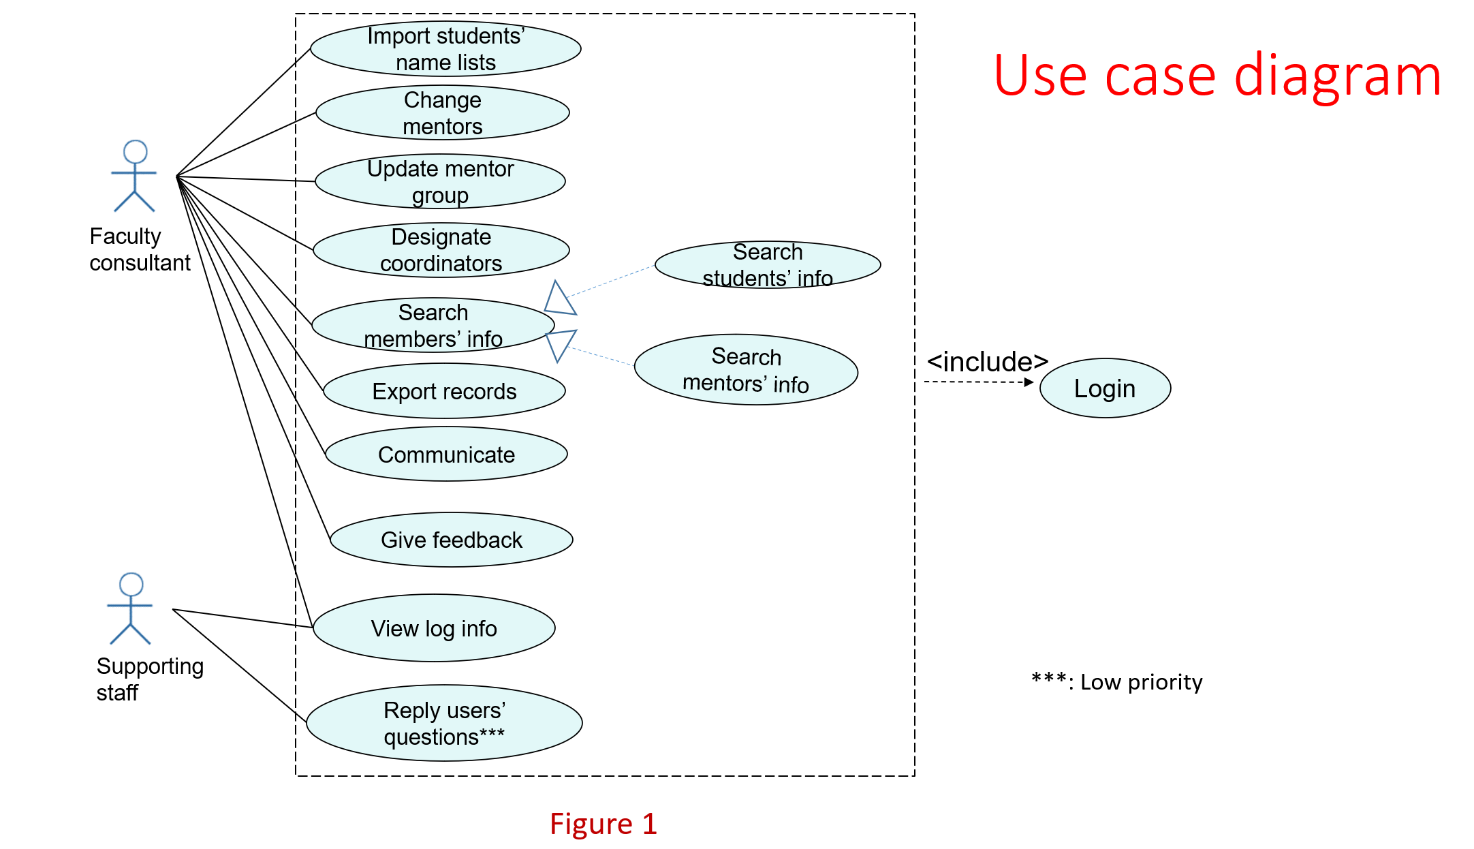
\includegraphics[width=\textwidth]{usecase_fig1.png}
\caption{Use Case Diagram: Mentor, Student and Coordinator}
\label{fig:main-usecase-fig1}
\end{figure}

\begin{figure}[htbp]
\centering
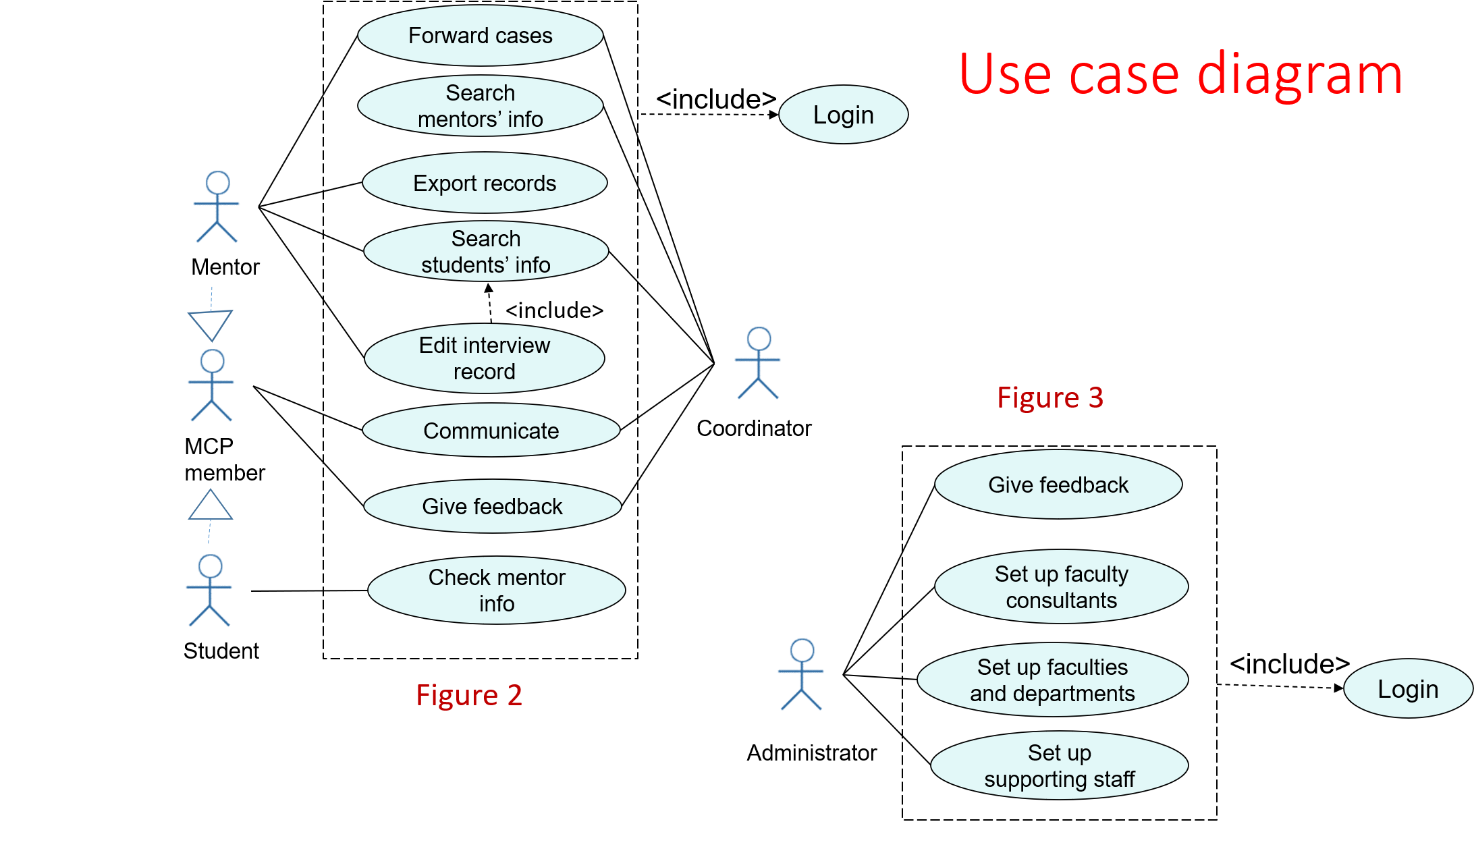
\includegraphics[width=\textwidth]{usecase_fig2_fig3.png}
\caption{Use Case Diagram: Administrator, Faculty Consultant and Supporting Staff}
\label{fig:main-usecase-fig2-fig3}
\end{figure}

\subsection{User Classes and Characteristics}

MCS is designed for six distinct user classes, differentiated by security/privilege levels, subset of product functions used and frequency of use, all of whom access the system via BNBU's unified account authentication. Core user classes and their pertinent characteristics are as follows, with faculty consultants and mentors as the favored user classes (the main daily operators of the system):

\begin{enumerate}
\item \textbf{Administrator}
\begin{itemize}
\item Privilege Level: Highest system privilege; only 1 user for the entire university.
\item Core Characteristics: Non-technical or technical background (BNBU school management staff); low frequency of system use (mainly for initial setup and occasional maintenance).
\item Key Functions: Designate/modify/delete faculty consultants, configure organizational architecture (faculty-department-major), set up supporting staff.
\item Unique Constraints: Cannot act as a mentor in the system.
\end{itemize}

\item \textbf{Faculty Consultant}
\begin{itemize}
\item Privilege Level: High; one or more per BNBU faculty (FST, FHSS, FSM, DCC).
\item Core Characteristics: Faculty management staff with familiarity with Excel operation; medium-to-high frequency of use (key operation at the start of each academic year, regular daily maintenance).
\item Key Functions: The core manager of the faculty-level MCS, responsible for mentor-student allocation import, group adjustment, MCP coordinator designation, multi-dimensional information search/export and cross-role communication.
\item Favored User Class: Primary daily operator of the system, core to the normal operation of the Mentor Caring Programme.
\end{itemize}

\item \textbf{Mentor}
\begin{itemize}
\item Privilege Level: Medium; assigned to mentor groups for undergraduate students.
\item Core Characteristics: BNBU teaching staff; high frequency of use (daily communication with students, interview record management, regular appointment arrangement).
\item Key Functions: Restricted to operating on their own supervised groups, including student information query, interview record editing, mentor-student communication/appointment, special case forwarding and interview record export.
\item Favored User Class: The most frequent operator of the system, the direct executor of the Mentor Caring Programme's core work.
\end{itemize}

\item \textbf{Student}
\begin{itemize}
\item Privilege Level: Low; all BNBU undergraduate students in mentor groups.
\item Core Characteristics: Non-technical background; variable use frequency (mainly for checking mentor information, responding to messages/appointments).
\item Key Functions: View personal mentor's basic information, two-way communication and interview appointment with the mentor.
\item Unique Constraints: Cannot access the system if not assigned to any mentor group (system displays a warning and forces logout).
\end{itemize}

\item \textbf{MCP Coordinator}
\begin{itemize}
\item Privilege Level: Medium; one per BNBU department, designated by faculty consultants.
\item Core Characteristics: Department management staff; medium frequency of use (mainly for special case forwarding and cross-role communication).
\item Key Functions: Search mentor/student information, forward student special cases from mentors to faculty consultants, and two-way communication with students, faculty consultants and mentors.
\item Flexible Attribute: May concurrently hold the role of a mentor for a mentor group.
\end{itemize}

\item \textbf{Supporting Staff}
\begin{itemize}
\item Privilege Level: Low; designated by the administrator (optional role).
\item Core Characteristics: School administrative staff; low frequency of use (auxiliary system management).
\item Key Functions: View all students' log information, respond to user feedback on system usage (the latter function is non-mandatory).
\end{itemize}
\end{enumerate}

\subsection{Operating Environment}

\textbf{Server-side Environment}

The Mentor Caring System (MCS) shall be deployed on a standard enterprise-level server capable of hosting a web application and a dedicated relational database. The server must maintain a stable network connection to the BNBU school database server for user identity verification and to the BNBU email server for automatic notification delivery. The specific server hardware configuration and operating system shall be determined during the system design phase based on the expected scale of university-wide usage.

\textbf{Recommended Configuration}

Hardware Platform: Enterprise-level server (CPU: Intel Xeon Silver/Gold or equivalent or above; RAM: 32GB or above; Hard Disk: 1TB SSD or above) with high-speed and stable network connectivity.

Operating System: Enterprise-grade Linux distribution (such as Rocky Linux 8/9 or Ubuntu Server 20.04/22.04 LTS) or Windows Server 2022 (64-bit).

Supporting Software: Relational database management system (MySQL 8.0 latest stable version / SQL Server 2019 or above); Web server (Nginx 1.20 or above / Apache Tomcat 9.0 or above).

\textbf{Client-side Environment}

\begin{sloppypar}
Users shall access the system through standard personal computers (desktops or laptops) equipped with mainstream modern web browsers. Client devices must have basic network access to the BNBU internal campus network, or external network access through the university's VPN\@ service. Users are also required to have Microsoft Excel (for importing and editing system-related data files as specified in Appendix A--D) and Microsoft Word (for viewing and editing exported report files) installed on their devices.
\end{sloppypar}

\textbf{Recommended Configuration}

Hardware Platform: Personal computer with Intel i5 / AMD Ryzen 5 or above, RAM 8GB or above, SSD storage and stable broadband network connection.

Operating System: Windows 11 (64-bit) or macOS 13 or above.

Browser: Latest stable versions of Chrome, Edge or Firefox.

Supporting Software: Microsoft Office 2019 / Microsoft 365 or above.

\textbf{Coexistence Requirements}

The system must peacefully coexist with the existing BNBU school database system and the school's email server (for sending system message notifications), without occupying excessive system resources or affecting the normal operation of other BNBU internal information systems.

\subsection{Design and Implementation Constraints}

The design and implementation of MCS are subject to the following constraints, which limit the development options for the development team:

\begin{enumerate}
\item \textbf{Functional Adaptability Constraint:} The system must support the dynamic addition of new faculties in BNBU without modifying the core code, to adapt to the school's future organizational structure adjustments.
\item \textbf{Data Retention Constraint:} All student information (including personal data, interview records, group history) must be permanently retained in the system; no data deletion is allowed for any operation (e.g., removing a student from a group, changing a group's mentor).
\item \textbf{Data Interaction Constraint:} The system can only read data from the BNBU school database (for user authentication) and cannot modify, delete or store any original data of the school database; all system-specific data (e.g., mentor-student allocation, interview records) must be stored in MCS's independent database.
\item \textbf{File Format Constraint:} The system must strictly support the Excel/Word file formats specified in the BNBU Mentor Caring Programme appendices (Appendix A-D) for data import and export; no custom non-standard file formats are allowed.
\item \textbf{Message Notification Constraint:} All system internal messages (e.g., communication, appointment) must trigger an automatic email notification to the receiver via the BNBU email server; receivers can only view and respond to messages after logging into the system.
\item \textbf{Appointment Time Constraint:} The mentor-student interview appointment function must set available time slots in 30-minute fixed intervals; no custom time slot durations are supported.
\item \textbf{Permission Isolation Constraint:} Mentors can only access and operate data related to their own supervised groups; no cross-group data access is allowed, and the system must strictly enforce role-based access control (RBAC) for all user classes.
\item \textbf{Maintainability Constraint:} The system code must follow standard software development programming norms (e.g., modular design, detailed code comments) to facilitate subsequent maintenance and version iteration by BNBU's technical staff.
\item \textbf{Excel Import Constraint:} When importing Excel files into the system, existing information in the system must not be overwritten; only non-existing information is updated, and the import logic must follow this rule for all Excel-based data operations.
\end{enumerate}

\subsection{User Documentation}

The following user documentation components will be delivered along with the MCS software, all complying with BNBU's internal information system documentation standards and the general software user manual writing norms. All documents will be provided in both electronic (PDF format) and editable (Word format) versions, and published on the BNBU internal system platform for easy access by all users:

\begin{enumerate}
\item \textbf{MCS Quick Start Guide:} A concise document for all user classes, including basic system access steps, account authentication instructions, core function operation shortcuts and common problem troubleshooting (1-2 pages for quick reference).

\item \textbf{MCS Detailed User Manual:} A comprehensive document classified by user roles, including detailed step-by-step operation instructions for all functions, screenshot demonstrations of key operations, file format specifications (Appendix A-D) and system error code explanations. Separate chapters are provided for each role to ensure targeted readability.

\item \textbf{MCS Administrator Maintenance Manual:} A dedicated document for the system administrator, including organizational architecture configuration, role permission setting, supporting staff management, system log viewing and basic system maintenance operations (e.g., data backup, Excel template update).

\item \textbf{MCS File Template Package:} A compressed package containing the standard Excel templates for Appendix A (organizational architecture), Appendix B (mentor-student allocation) and Appendix C (MCP coordinator designation), with built-in data validation rules to ensure user input compliance.
\end{enumerate}

\subsection{Assumptions and Dependencies}

\textbf{Assumptions}

The following assumed factors (not yet verified as absolute facts) affect the requirements and implementation of MCS; if these assumptions are incorrect, unshared or changed, the project development and system operation will be impacted:

\begin{enumerate}
\item The BNBU school database is permanently available and stably connected during the entire operation period of MCS, and provides a fixed data interface for MCS to read user account, password, name and role information.
\item The BNBU email server is always operational and supports the system's automatic email notification function; the server has no sending frequency or content restrictions for internal school email notifications.
\item All MCS users (especially faculty consultants and mentors) have basic computer operation skills and are proficient in using Microsoft Excel and Word (the core office software for the system).
\item BNBU will not adjust the core attributes of the user account (e.g., student ID, staff email) during the system operation period; any account attribute adjustment will be notified to the development team in advance.
\item The non-mandatory function of ``supporting staff responding to user feedback'' will not require additional integration with BNBU's feedback system; the supporting staff only needs to process feedback via manual record within MCS.
\end{enumerate}

\textbf{Dependencies}

The development and operation of MCS have the following key external dependencies, which are essential for the realization of core system functions:

\begin{enumerate}
\item \textbf{BNBU School Database Interface:} The system is dependent on the provision of a valid, read-only data interface by the BNBU Information Technology Center; without this interface, the unified user identity authentication function cannot be realized.
\item \textbf{BNBU Email Server Service:} The system is dependent on the BNBU email server to provide SMTP/POP3 services for automatic message notification; the interruption of this service will result in the failure of the email notification function for communication and appointments.
\item \textbf{Microsoft Office Software:} The system's data import/export function is dependent on the mainstream Microsoft Office (Excel/Word) software used by all BNBU users; the system does not support other office software with incompatible file formats.
\item \textbf{BNBU Internal Network Environment:} The system's core data interaction (e.g., accessing the school database) is dependent on the stability of the BNBU internal campus network; external network access requires the school's VPN service to ensure secure and stable connection to the system server.
\end{enumerate}

%--------------------------------------------------------------
% 3. Use Case
%--------------------------------------------------------------
% Section 3: Use Case
\section{Use Case}

%--------------------------------------------------------------
\subsection{Check Mentor Info}

\subsubsection{Description and Priority}

This feature enables a student to check the assigned mentor's information after logging into the system. The displayed information includes the mentor's basic profile relevant to the student's mentoring arrangement.

Priority: Medium

\begin{figure}[H]
\centering
\includegraphics[width=\textwidth]{"Figure 2_1.pdf"}
\caption{Transition diagram for Check Mentor Info}
\label{fig:check-mentor-info}
\end{figure}

\subsubsection{Stimulus/Response Sequences}

Scenario:

Actor: Student

Assumption: The user has already logged into the system and is currently on the 1B. Home Page student.

Main Success Scenario:
\begin{enumerate}
\item The user clicks the ``Check Mentor Info'' button on the 1B. Home Page student.
\item The system verifies that the student belongs to a mentor group.
\item The system transitions to and displays the 3D. Mentor Info Page.
\item The user views the assigned mentor's information.
\end{enumerate}

Alternative Flows:

1a. If the student does not belong to any mentor group, the system does not enter the Mentor Info Page and displays a corresponding warning message.

\subsubsection{Functional Requirements}

REQ-1: The system shall allow only a student belonging to a valid mentor group to access the mentor information page.

REQ-2: The system shall display the assigned mentor's relevant information in read-only form.

REQ-3: The system shall prevent the student from modifying any mentor information on this page.

%--------------------------------------------------------------
\subsection{Search Student's Info}

\subsubsection{Description and Priority}

This feature enables Mentor and MCP Coordinator to search for a student's full information in the system by inputting the unique student ID. The system will display the student's core information (including Student ID, Group ID, Mentor name, Faculty/Department/Major, and status) and all associated interview records of the student. This feature is a mandatory prerequisite for the ``Edit Interview Record'' function (3.3) for Mentors, and is the basic function for daily student information management for both roles.

Priority: High

\subsubsection{Stimulus/Response Sequences}

Transition diagram is included in 3.3.2.

Scenario:

Actor: Mentor, MCP Coordinator

Assumption: The user has successfully logged into the system.

Main Success Scenario:
\begin{enumerate}
\item The user selects the ``Search Student Info'' function.
\item The system prompts the user to enter a Student ID.
\item The user enters a valid Student ID and clicks ``Search''.
\item The system retrieves the data and displays the student's detailed information and interview records.
\end{enumerate}

Alternative Flows:

3a. If the Student ID does not exist, or if the user does not have permission, the system displays an error prompt.

\subsubsection{Functional Requirements}

REQ-1: The system shall perform real-time format verification on the input student ID; if the format is invalid, the system shall reject the input at the backend.

REQ-2: The system shall strictly restrict Mentors to only retrieve and view student information belonging to their own assigned mentoring group during their active duty period.

REQ-3: The system shall restrict MCP Coordinators to only retrieve and view student information belonging to their own department.

%--------------------------------------------------------------
\subsection{Edit Interview Record}

\subsubsection{Description and Priority}

The mentor can click Edit to add, modify or delete the interview record. If the record exists, it can be modified or deleted; if empty, a new record can be entered.

Priority: High

Remark: Combined transition diagram for Search Student's Info (3.2) and Edit Interview Record (3.3). Coordinator can view the Student's info but cannot edit it; Mentor can do both.

\begin{figure}[htbp]
\centering
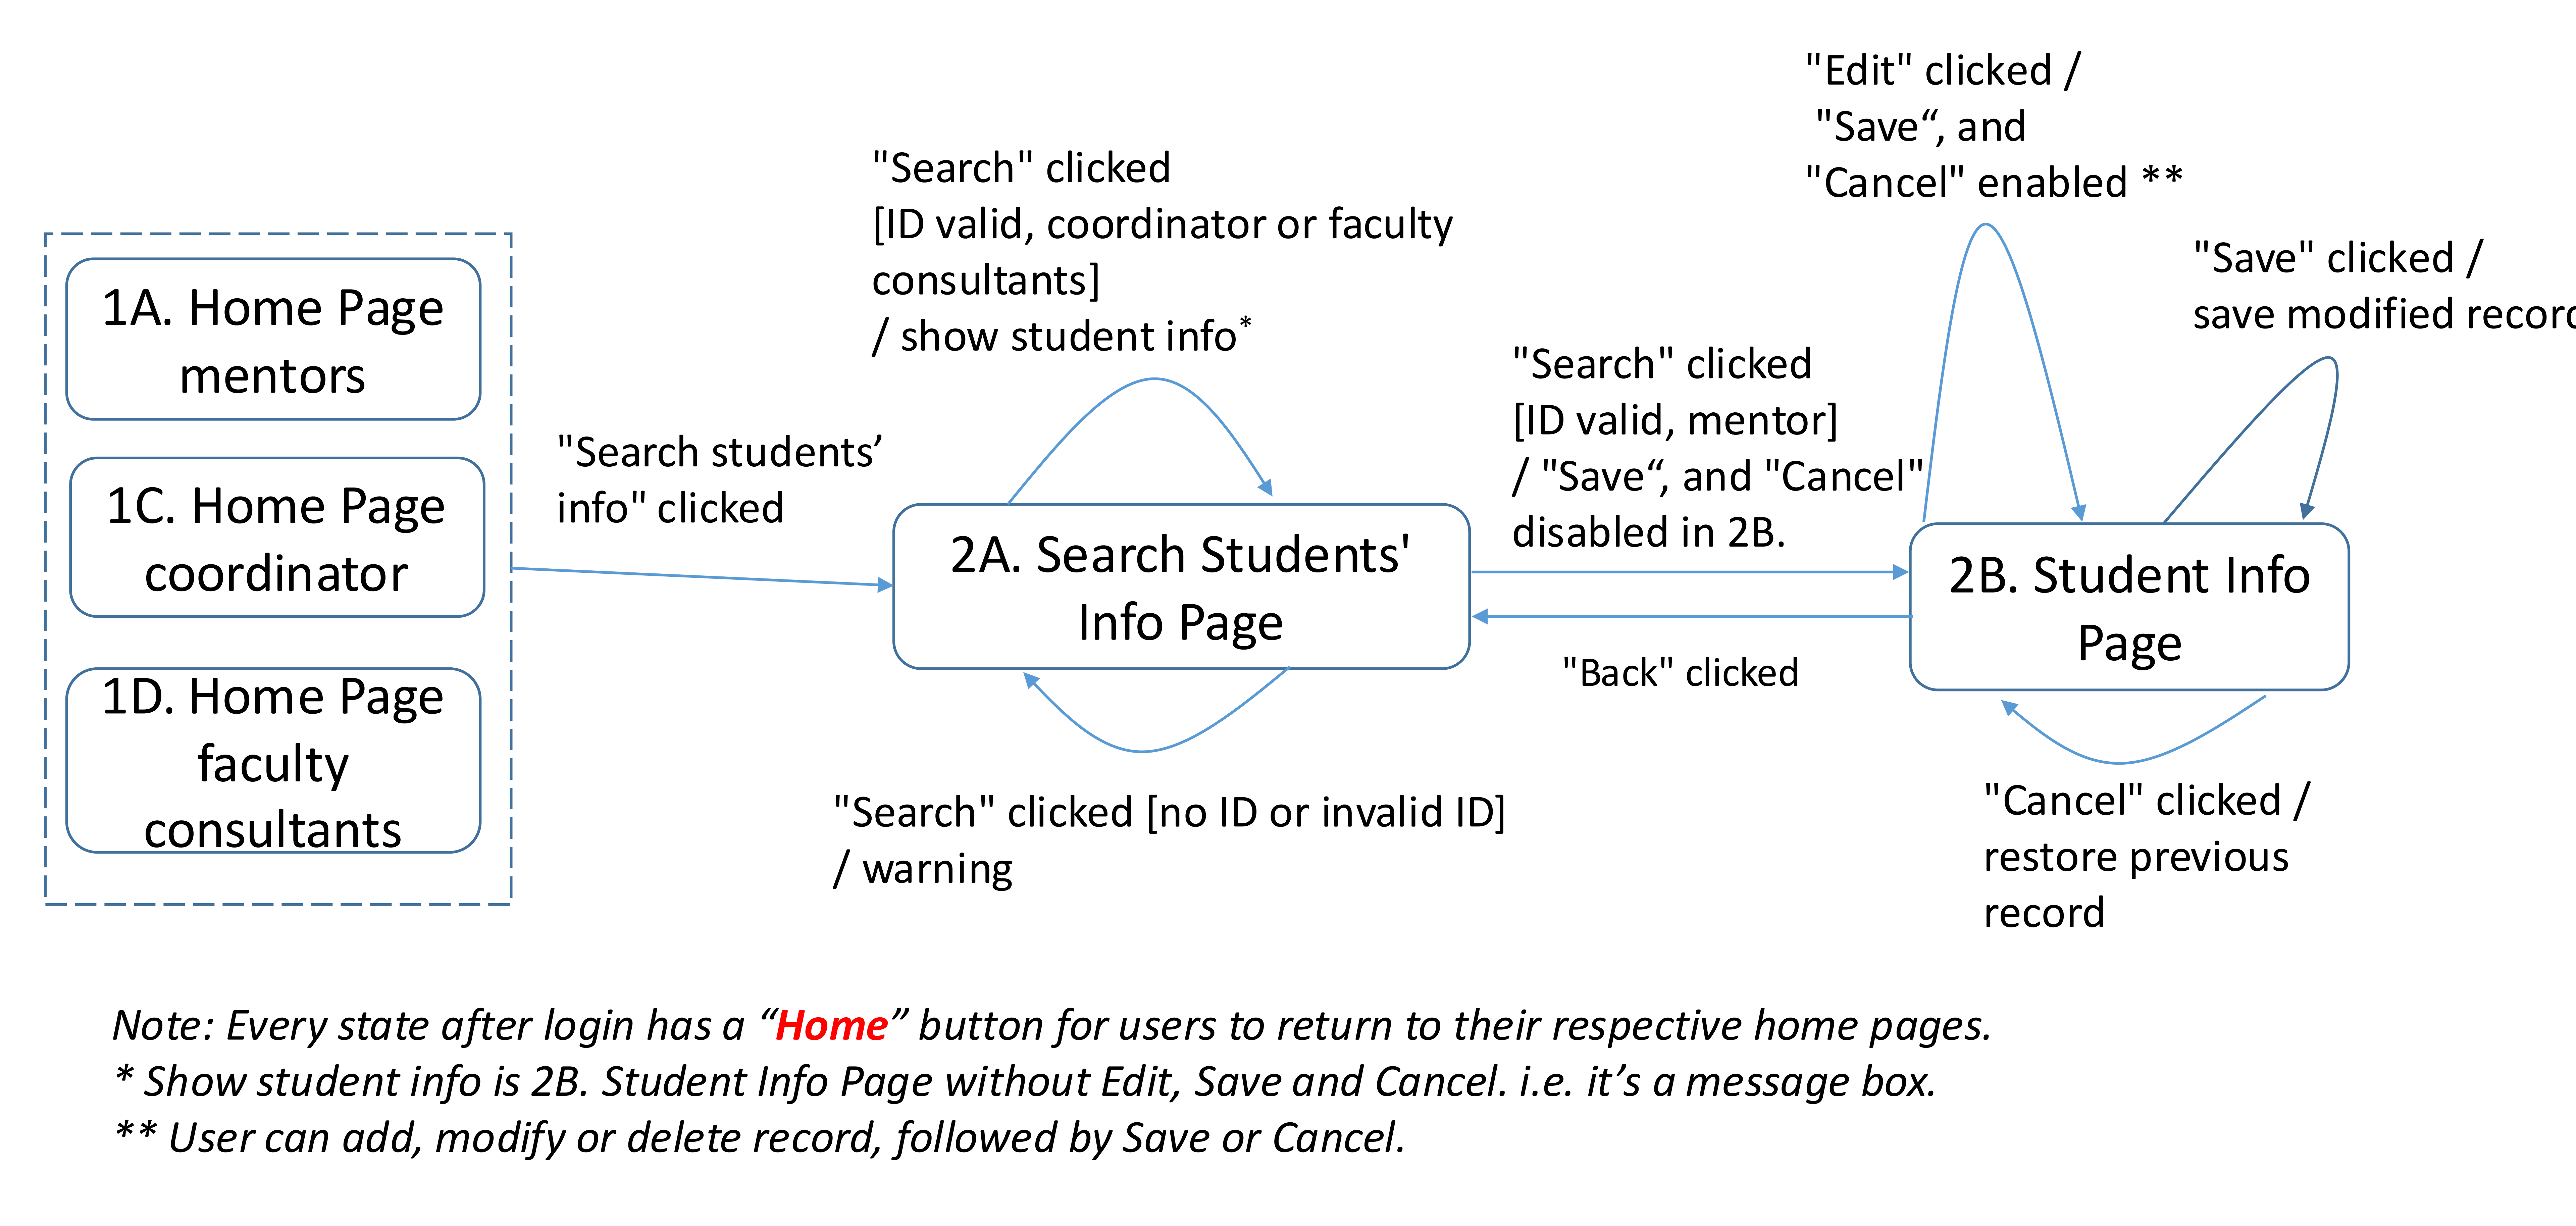
\includegraphics[width=\textwidth]{std_search_edit.png}
\caption{Transition diagram for Search Student's Info and Edit Interview Record}
\label{fig:search-edit-interview-record}
\end{figure}

\subsubsection{Stimulus/Response Sequences}

Scenario:

Actor: Mentor

Assumption: Search Student Info must be performed first. The mentor is currently in a student's info page.

Main Success Scenario:
\begin{enumerate}
\setcounter{enumi}{4}
\item The Mentor clicks the ``Edit'' button on the 2B. Student Info Page.
\item The system transitions to the 2B2. Interview Record Form. If an interview record exists, the current text is displayed; if it is empty, blank input fields are displayed.
\item The Mentor enters a new record, modifies the existing record, or deletes the record.
\item The Mentor clicks the ``Save'' button.
\item The system saves the changes and returns to the updated 2B. Student Info Page.
\end{enumerate}

Alternative Flows:

4a. If the Mentor clicks ``Cancel'' instead of ``Save'', the system discards any changes and returns to the 2B. Student Info Page.

\subsubsection{Functional Requirements}

REQ-1: The system backend must validate that all mandatory fields are not empty before executing the save command and writing the interview record into the database.

REQ-2: The system must automatically append a hidden timestamp and the operator's Mentor ID to the database record every time an interview record is successfully created or modified, for backend tracking purposes.

%--------------------------------------------------------------
\subsection{Search Mentor's Info}

\subsubsection{Description and Priority}

Search for a mentor info, given a mentor's name, email address or group ID. The search result includes the mentor's name and ID of the group for which the mentor cares. The member list is displayed by clicking on the group ID. The record of a student is shown by selecting the name of the student in the member list.

Priority: Low

\begin{figure}[htbp]
\centering
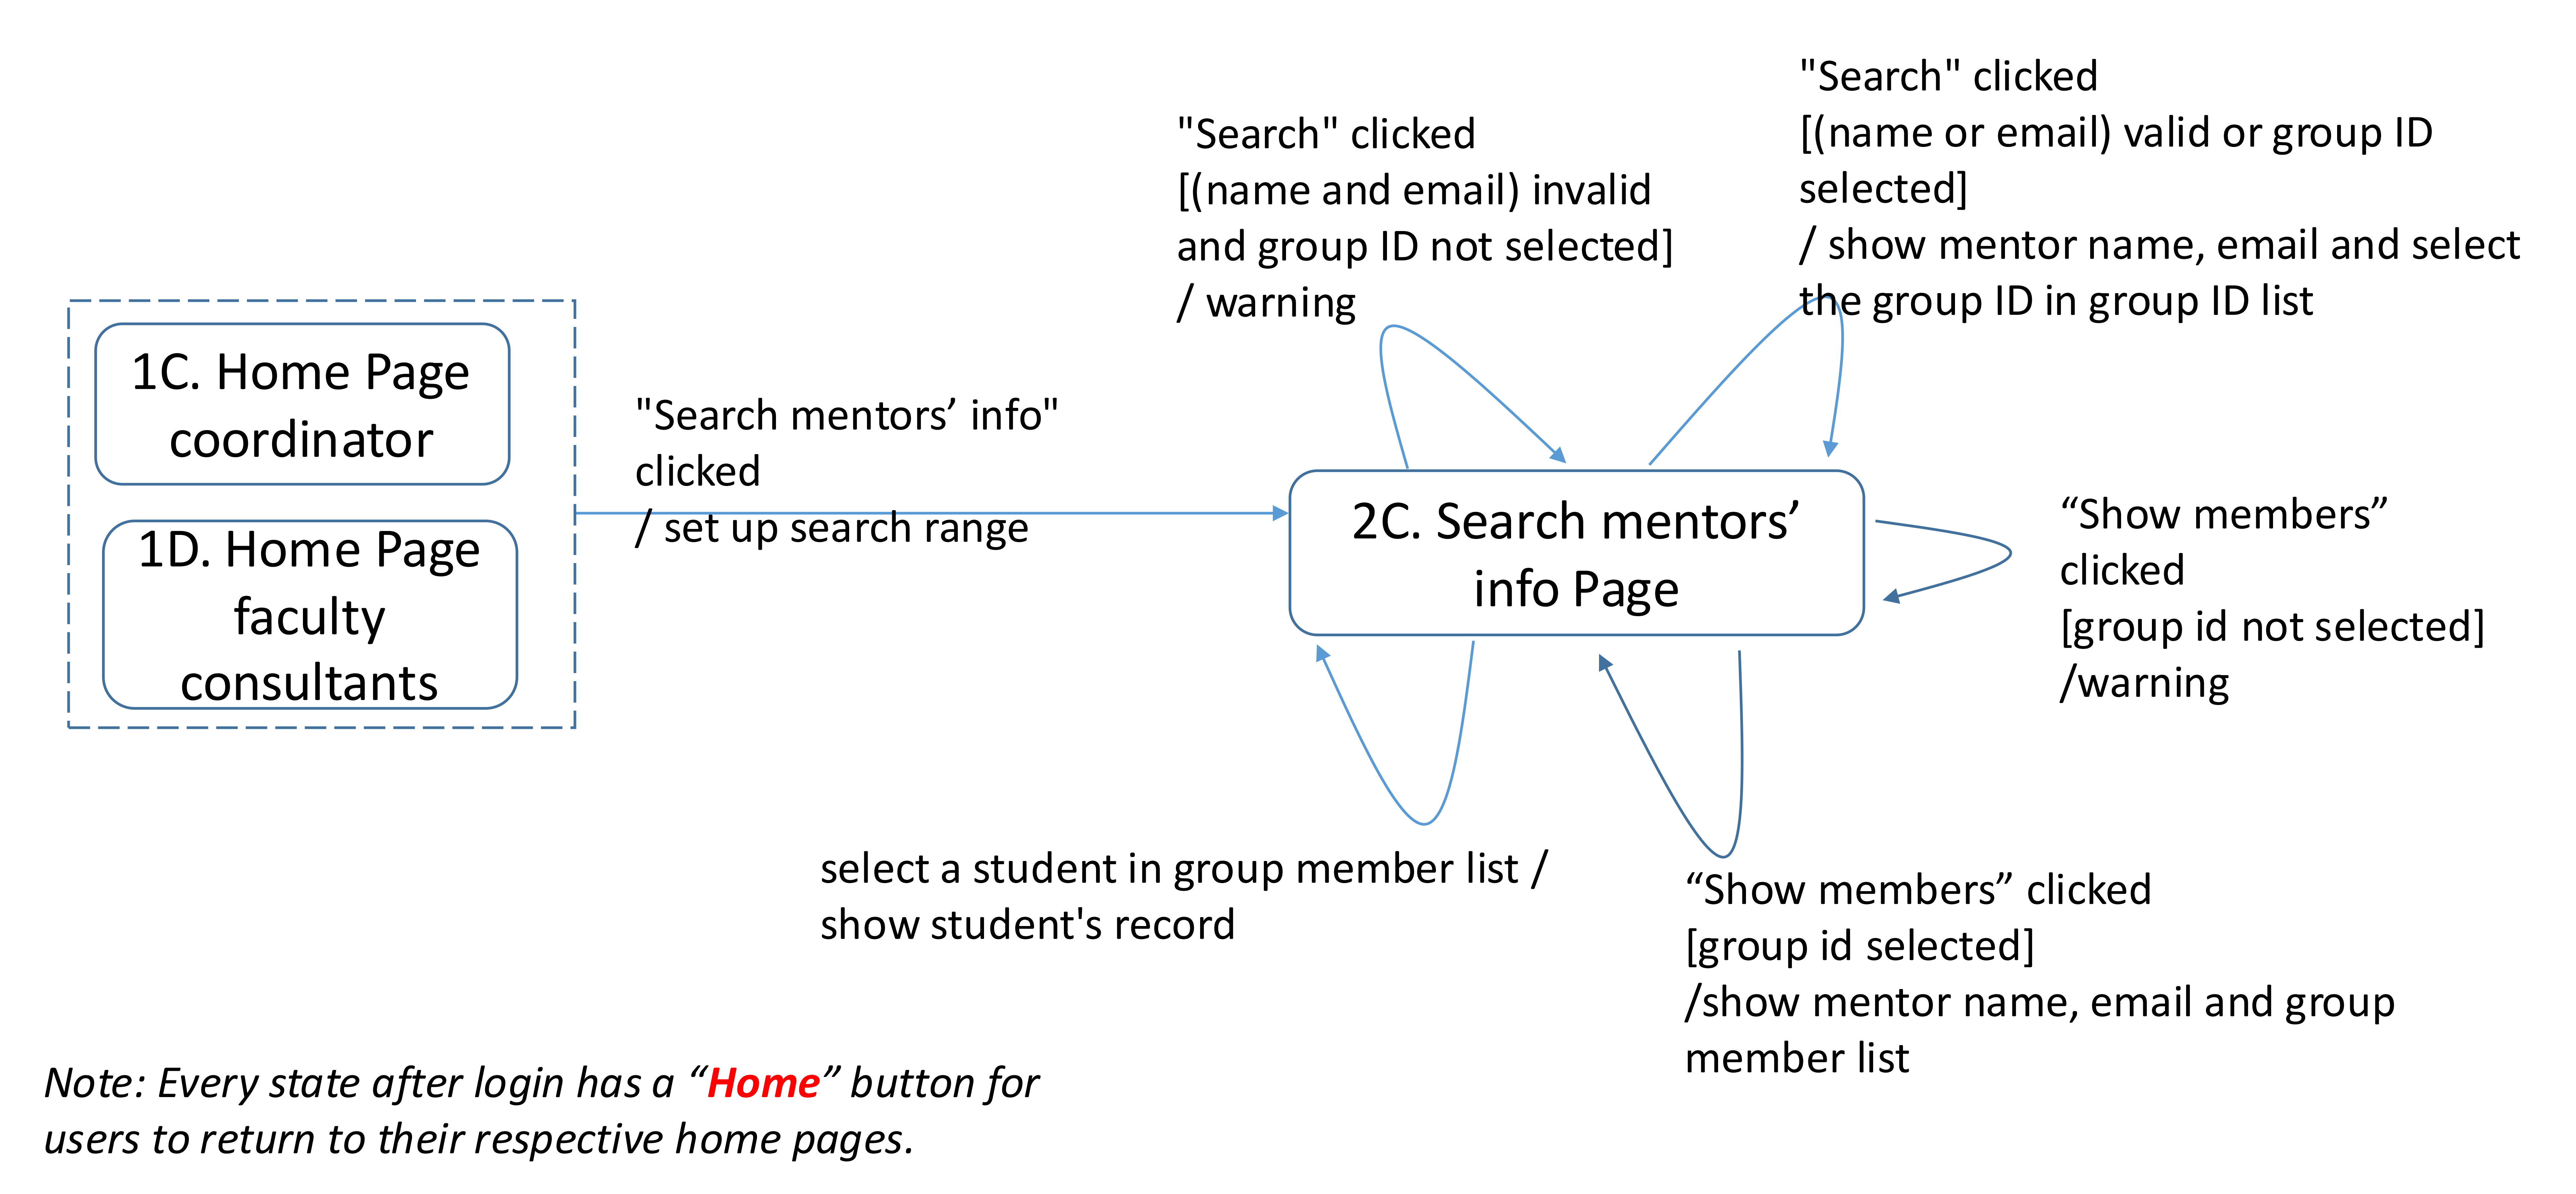
\includegraphics[width=\textwidth]{std_search_mentor.png}
\caption{Transition diagram for Search Mentor's Info}
\label{fig:search-mentor-info}
\end{figure}

\subsubsection{Stimulus/Response Sequences}

Scenario:

Actor: Faculty Consultant, Coordinator

Assumption: The user has already logged into the system and is currently on the 2C. Search Mentors' Info Page.

Main Success Scenario:
\begin{enumerate}
\item The user enters a mentor name, email address or group ID on the 2C. Search Mentors' Info Page.
\item The user clicks the ``Search'' button.
\item The system searches for mentor information based on the input condition.
\item The system displays the search results on the 2C. Search Mentors' Info Page, including the mentor's name and the list of group IDs.
\item The user clicks a group ID.
\item The system displays the student list of that group on the 2C1. Group Members Page.
\item The user selects a student from the list.
\item The system displays the record of the selected student on the 2B. Student Info Page.
\end{enumerate}

Alternative Flows:

4a. If no matching mentor is found, the system informs the user that no matching result is found and asks the user to enter another search condition.

6a. If there is no student in the selected group, the system displays an empty student list.

8a. If the selected student has no record, the system informs the user that no record is available for that student.

\subsubsection{Functional Requirements}

REQ-1: The system shall support flexible backend matching algorithms allowing searches using partial or complete input of mentor name, email address, or group ID.

REQ-2: The system must retain and display all historical information of students when their records are accessed, even if they have been removed from a group or their mentor has changed.

%--------------------------------------------------------------
\subsection{Import Students' Name Lists}

\subsubsection{Description and Priority}

This feature enables a Faculty Consultant to import students' name lists into the system through an Excel file. The system validates the file format, previews the uploaded data and updates the database without overwriting existing records.

Priority: High

\begin{figure}[H]
\centering
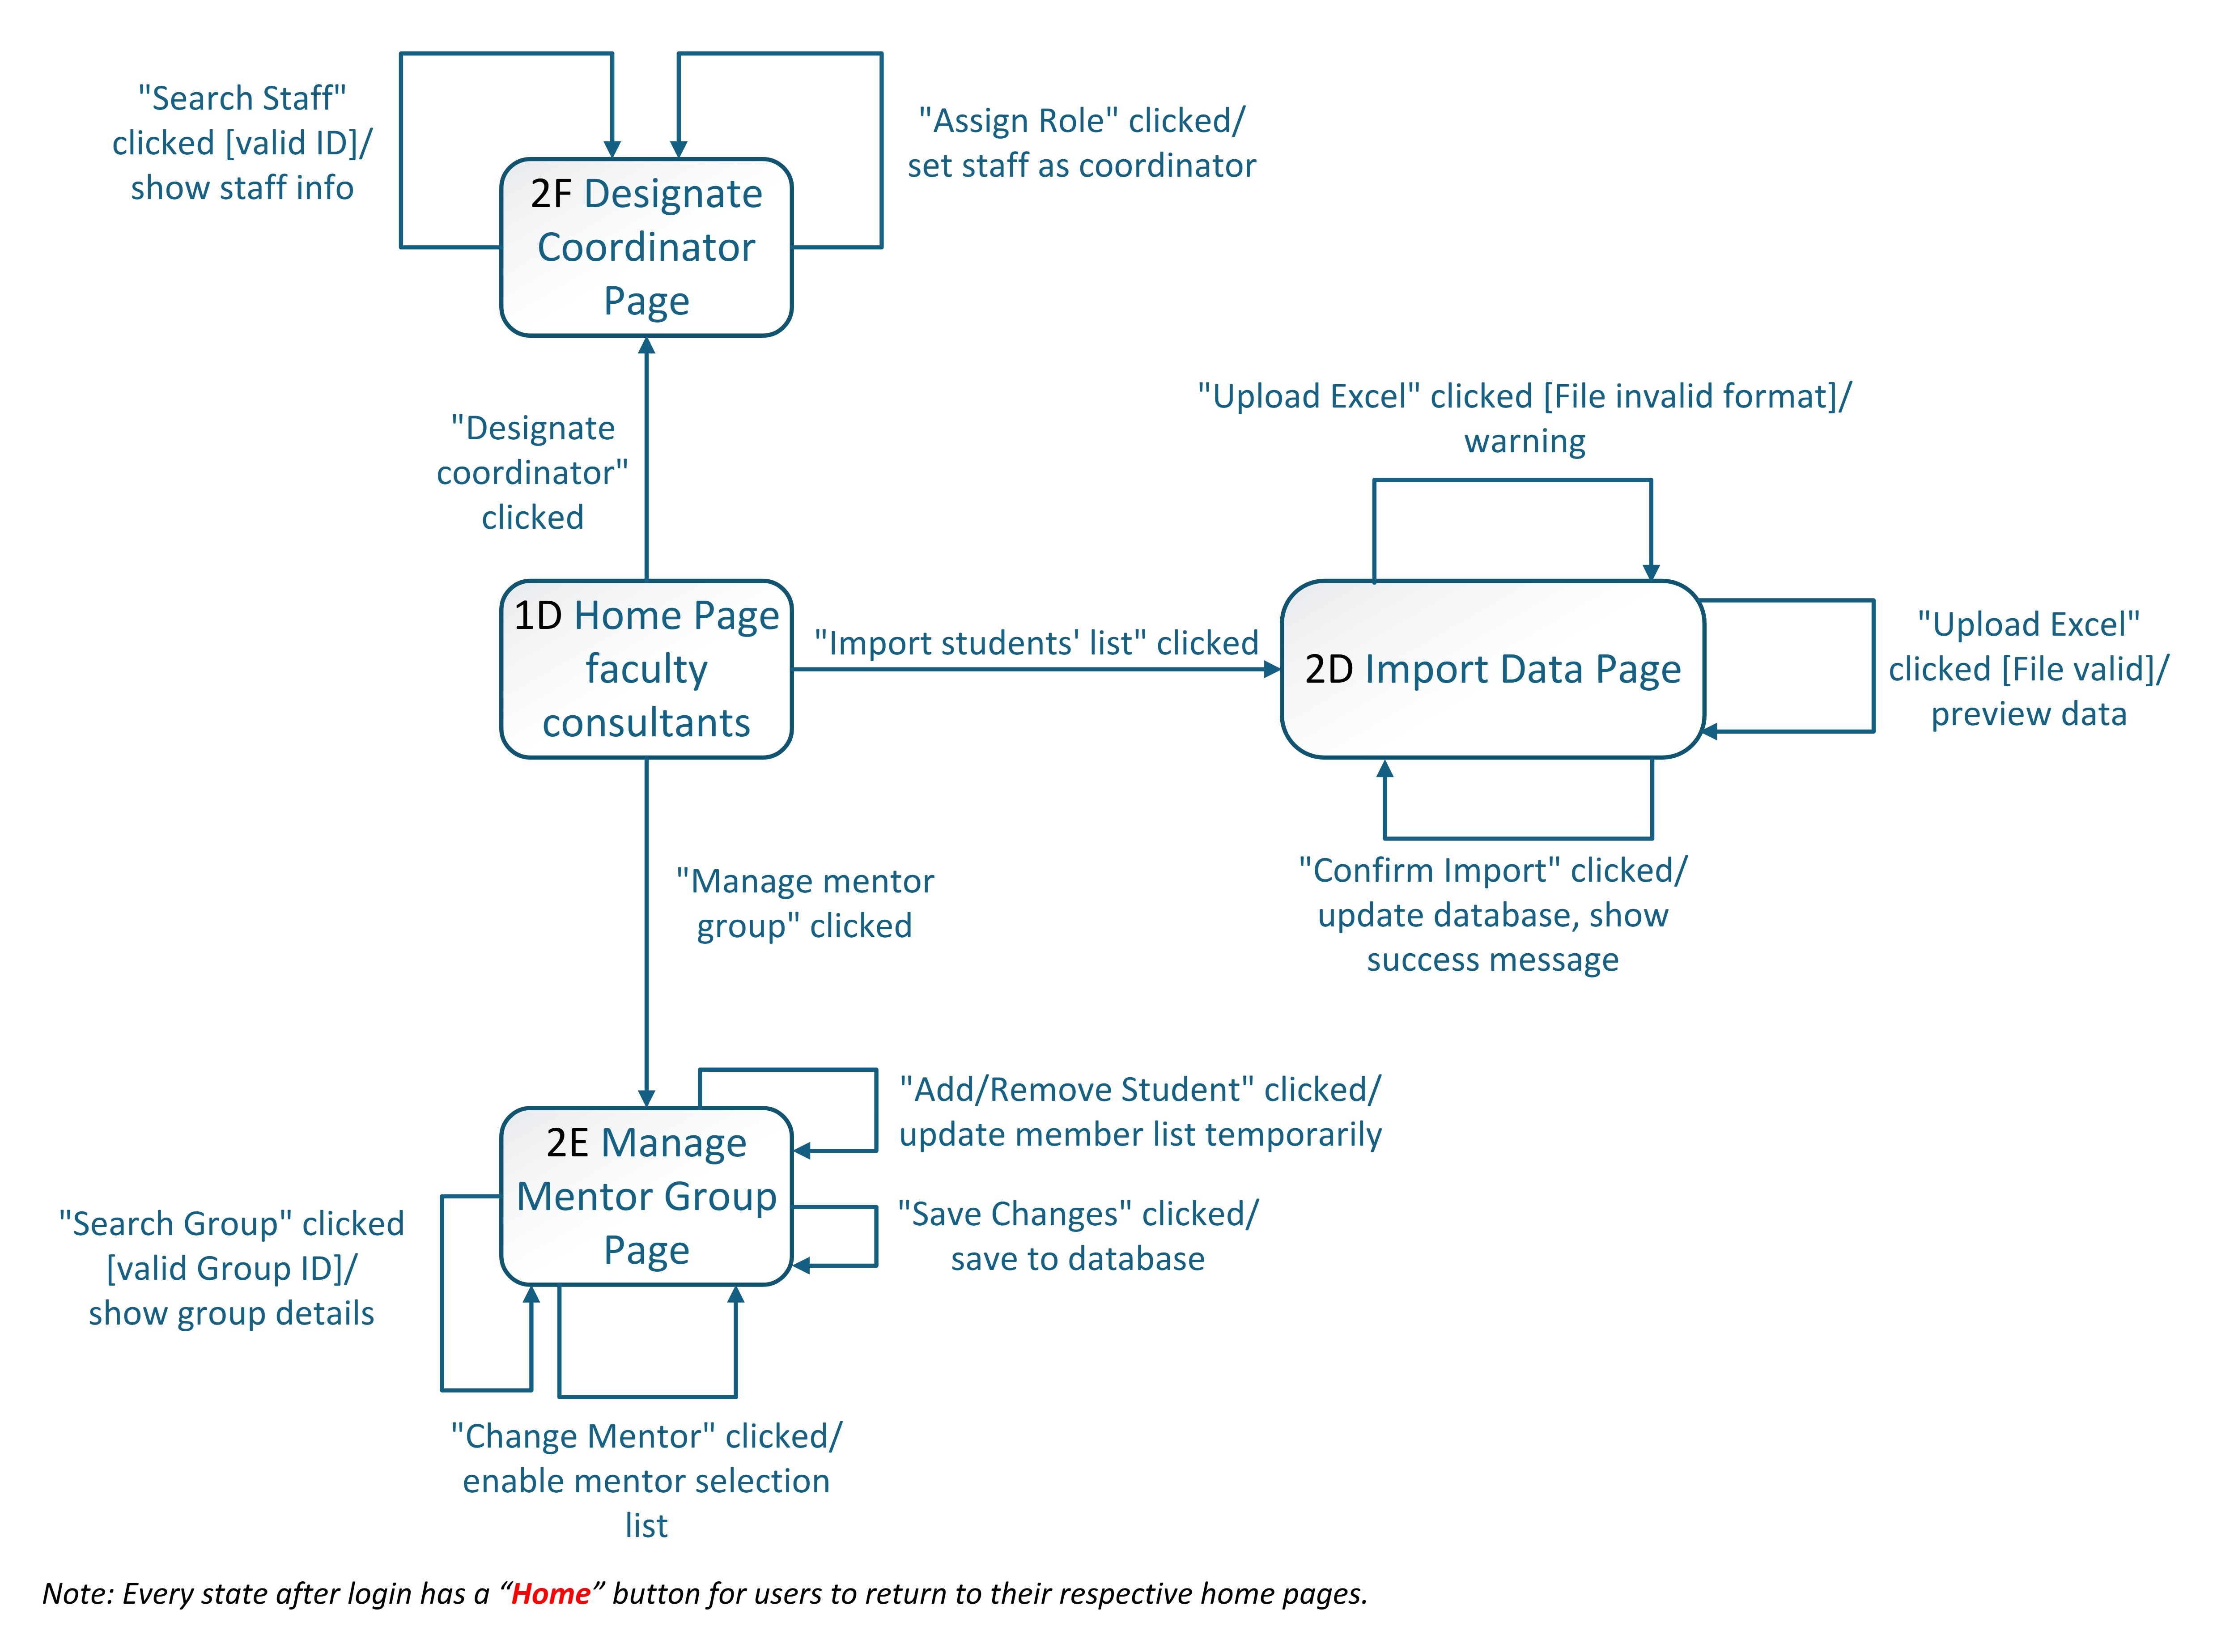
\includegraphics[width=\textwidth]{Page_3_docsmall.com.jpg}
\caption{Transition diagram for Faculty Consultant management functions}
\label{fig:faculty-consultant-functions-import}
\end{figure}

\subsubsection{Stimulus/Response Sequences}

Scenario 1: Import Students' Name Lists

Actor: Faculty Consultant

Assumption: The user has already logged into the system and is currently on the 1D. Home Page faculty consultants.

Main Success Scenario:
\begin{enumerate}
\item User clicks the ``Import students' list'' button on the 1D. Home Page faculty consultants.
\item System transitions to and displays the 2D. Import Data Page.
\item User clicks ``Upload Excel'', selects a valid Excel file containing the students' name lists, and uploads it.
\item System validates the file format (must be Excel) and displays a preview of the uploaded data in the display area.
\item User clicks the ``Confirm Import'' button.
\item System updates the database with new information without overwriting existing data, and displays a success message.
\end{enumerate}

Alternative Flows:

3a. If the uploaded file is not in valid Excel format, the system displays a warning message and remains on the 2D. Import Data Page.

4a. If the uploaded data contains invalid or incomplete records, the system marks the problematic entries and prevents final import until the errors are corrected.

\subsubsection{Functional Requirements}

REQ-1: The system shall accept only Excel files conforming to the required import template.

REQ-2: The system shall validate the uploaded file format before displaying a data preview.

REQ-3: The system shall provide a preview of uploaded data before database update.

REQ-4: The system shall update only non-existing information and shall not overwrite existing data.

REQ-5: The system shall record each import operation in the system log.

%--------------------------------------------------------------
\subsection{Manage Mentor Group}

\subsubsection{Description and Priority}

This feature enables a Faculty Consultant to search for a mentor group, review group details, change the assigned mentor and save the updated group information while preserving historical data.

Priority: High

\subsubsection{Stimulus/Response Sequences}

Transition diagram is included in 3.5.2.

Scenario 2: Manage Mentor Group

Actor: Faculty Consultant

Assumption: The user has already logged into the system and is currently on the 1D. Home Page faculty consultants.

Main Success Scenario:
\begin{enumerate}
\item User clicks the ``Manage mentor group'' button on the 1D. Home Page faculty consultants.
\item System transitions to and displays the 2E. Manage Mentor Group Page.
\item User enters a valid Group ID in the text input field and clicks the ``Search Group'' button.
\item System retrieves and displays the group details, including the current mentor and the student member list.
\item User selects a new mentor from the dropdown list and clicks the ``Change Mentor'' button.
\item System temporarily updates the mentor selection on the interface.
\item User clicks the ``Save Changes'' button.
\item System saves the changes to the database while permanently retaining all historical information of the students and displays a success confirmation.
\end{enumerate}

Alternative Flows:

3a. If the Group ID is invalid or does not exist, the system displays a warning message and remains on the 2E. Manage Mentor Group Page.

5a. If the selected mentor is not eligible for the group, the system rejects the change and displays an error message.

5b. User clicks the ``Add/Remove Student'' button to add a new student to or remove an existing student from the group.

6b. System temporarily updates the member list on the interface.

5c. If the user attempts to add a student who does not exist in the system, the system displays a warning.

7a. If the user leaves the page without saving, the system discards temporary changes.

\subsubsection{Functional Requirements}

REQ-1: The system shall allow only Faculty Consultants to manage mentor groups within their permitted scope.

REQ-2: The system shall support searching groups by Group ID and displaying group details.

REQ-3: The system shall allow Faculty Consultants to change the assigned mentor of a group.

REQ-4: The system shall preserve all historical student and mentor allocation information after each saved adjustment.

REQ-5: The system shall save only confirmed changes to the database.

%--------------------------------------------------------------
\subsection{Designate Coordinators}

\subsubsection{Description and Priority}

This feature enables a Faculty Consultant to search for a valid staff member and assign the MCP Coordinator role.

Priority: High

\subsubsection{Stimulus/Response Sequences}

Transition diagram is included in 3.5.2.

Scenario 3: Designate Coordinators

Actor: Faculty Consultant

Assumption: The user has already logged into the system and is currently on the 1D. Home Page faculty consultants.

Main Success Scenario:
\begin{enumerate}
\item User clicks the ``Designate coordinator'' button on the 1D. Home Page faculty consultants.
\item System transitions to and displays the 2F. Designate Coordinator Page.
\item User enters a valid Staff ID or Name in the search field and clicks the ``Search Staff'' button.
\item System retrieves and displays the staff member's basic information.
\item User clicks the ``Assign Role'' button.
\item System updates the staff member's role permissions to MCP Coordinator in the database and displays a success message.
\end{enumerate}

Alternative Flows:

3a. If the entered Staff ID or Name is invalid or no matching staff member is found, the system displays a warning message.

5a. If the staff member is outside the Faculty Consultant's permitted scope, the system denies the role assignment and displays an authorization error.

\subsubsection{Functional Requirements}

REQ-1: The system shall allow only Faculty Consultants to designate MCP Coordinators.

REQ-2: The system shall validate that the searched staff member exists and is within the permitted scope.

REQ-3: The system shall update the selected staff member's role to MCP Coordinator after a valid assignment.

REQ-4: The system shall record the role assignment action in the system log.

%--------------------------------------------------------------
\subsection{Export Records}

\subsubsection{Description and Priority}

This feature enables a Mentor or Faculty Consultant to export records based on selected criteria into a Microsoft Word file.

Priority: High

\begin{figure}[H]
\centering
\includegraphics[width=\textwidth]{"Figure 2_2.pdf"}
\caption{Detailed transition diagram for Export Records}
\label{fig:export-records-detail}
\end{figure}

\subsubsection{Stimulus/Response Sequences}

Scenario 4: Export Records

Actor: Mentor or Faculty Consultant

Assumption: The user has already logged into the system and is currently on their respective Home Page (1A or 1D).

Main Success Scenario:
\begin{enumerate}
\item User clicks the ``Export records'' button on their Home Page.
\item System transitions to and displays the 2G. Export Records Page.
\item User selects the valid Academic Year and Department from the dropdown boxes, optionally enters Mentor Name and/or Student Name, and clicks the ``Generate Document'' button.
\item System compiles the requested interview records and information into a Microsoft Word file format and triggers the file download.
\end{enumerate}

Alternative Flows:

3a. If required criteria are missing, the system displays a warning message and remains on the 2G. Export Records Page.

4a. If the system encounters an internal error during document generation, it displays an error message and prompts the user to try again later.

\subsubsection{Functional Requirements}

REQ-1: The system shall allow only authorized users to export records within their permitted scope.

REQ-2: The system shall support filtering exported records by Academic Year, Department, Mentor Name, and Student Name.

REQ-3: The system shall generate the export file in Microsoft Word format.

REQ-4: The system shall stop export and display a warning if required criteria are missing.

REQ-5: The system shall log each export operation for auditing purposes.

%--------------------------------------------------------------
\subsection{Communicate}

\subsubsection{Description and Priority}

This feature enables a Faculty Consultant, Mentor, MCP Coordinator or Student to send messages through the system and trigger an automatic email notification to the receiver.

Priority: High

\begin{figure}[H]
\centering
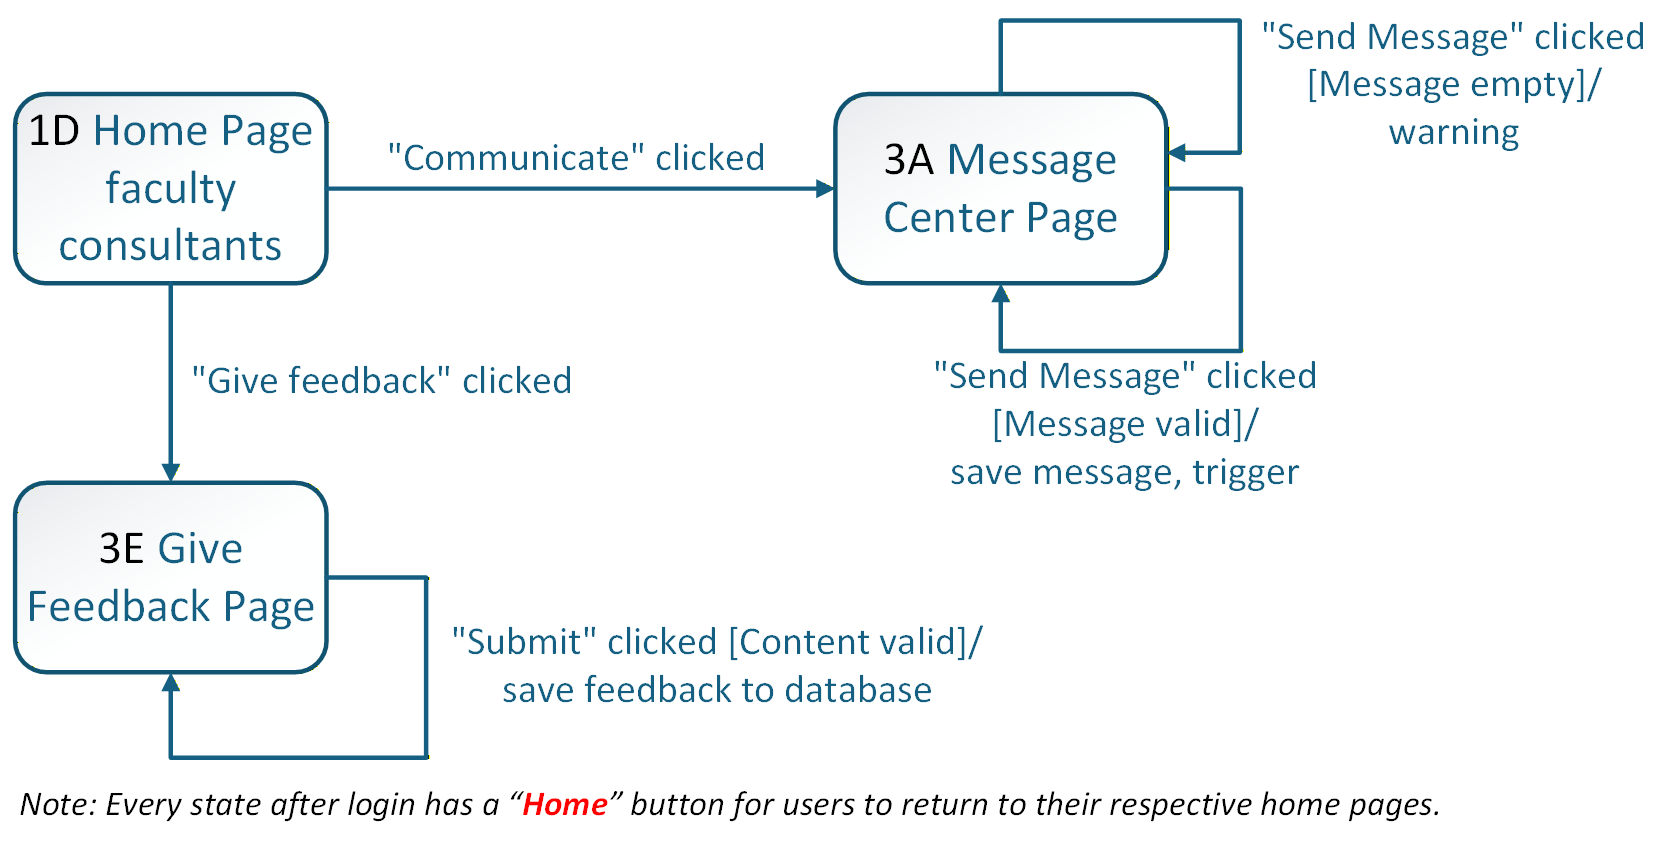
\includegraphics[width=\textwidth]{Page_5_docsmall.com.png}
\caption{Overview transition diagram for Communication and Give Feedback}
\label{fig:communicate-overview}
\end{figure}

\begin{figure}[H]
\centering
\includegraphics[width=\textwidth]{"Figure 2_3a.pdf"}
\caption{Detailed transition diagram for Send Message}
\label{fig:communicate-detail}
\end{figure}

\subsubsection{Stimulus/Response Sequences}

Scenario 5: Communicate

Actor: Faculty Consultant (or Mentor/Coordinator/Student)

Assumption: The user has already logged into the system and is currently on their Home Page.

Main Success Scenario:
\begin{enumerate}
\item User clicks the ``Communicate'' button on their Home Page.
\item System transitions to and displays the 3A. Message Center Page, showing the list of existing conversations.
\item User clicks on an existing conversation or clicks ``New Message''.
\item If an existing conversation is selected, the system displays the 3A1. Conversation Page with the message history.
\item If ``New Message'' is clicked, the system displays the 3A2. New Message Page.
\item On the 3A1. Conversation Page, user enters a message and clicks ``Send''.
\item On the 3A2. New Message Page, user selects a receiver from the list, enters a message, and clicks ``Send''.
\item System saves the message to the database, triggers an automatic email notification to the receiver via the BNBU email server, and displays a success message.
\end{enumerate}

Alternative Flows:

3a. If there are no existing conversations, the 3A. Message Center Page displays an empty list with an option to create a new message.

6a. If the message content is empty on 3A1. Conversation Page, the system displays a validation error and does not send the message.

7a. If the receiver is not selected on 3A2. New Message Page or the message content is empty, the system displays a validation error and does not send the message.

8a. If the email notification fails, the system still saves the message in the database but displays a warning that the email notification failed.

\subsubsection{Functional Requirements}

REQ-1: The system shall allow authorized users to send messages to permitted receivers according to role permissions.

REQ-2: The system shall display a list of existing conversations on the 3A. Message Center Page.

REQ-3: The system shall allow users to view message history in the 3A1. Conversation Page.

REQ-4: The system shall allow users to create new messages via the 3A2. New Message Page.

REQ-5: The system shall validate that the receiver is selected and the message content is not empty on the appropriate page.

REQ-6: The system shall save successfully submitted messages in the database.

REQ-7: The system shall trigger an automatic email notification after a message is saved.

REQ-8: The system shall notify the sender if email delivery fails while the internal message is saved successfully.

%--------------------------------------------------------------
\subsection{Make Appointment}

\subsubsection{Description and Priority}

This feature enables a Mentor to create interview appointment requests for students and enables the student to confirm a selected time slot.

Priority: High

\begin{figure}[H]
\centering
\includegraphics[width=\textwidth]{"Figure 2_3b.pdf"}
\caption{Transition diagram for Make Appointment}
\label{fig:make-appointment}
\end{figure}

\subsubsection{Stimulus/Response Sequences}

Scenario:

Actor: Mentor (Main), Student (Secondary)

Assumption: Mentor has logged in and is on 1A. Home Page mentor.

Main Success Scenario:
\begin{enumerate}
\item The Mentor clicks ``Make Appointment'' on the Home Page.
\item The system displays the 3B. Make Appointment Page with student selection and time slot options.
\item The Mentor selects a student and marks available 30-minute time slots.
\item The Mentor clicks ``Send Request''.
\item The system sends the request and waits for student response.
\item The student logs in, opens the 3B2. Select Time Slot Page, selects one slot and clicks ``Confirm''.
\item The system notifies the Mentor.
\item The Mentor opens the 3B1. Appointment Confirmation Page, enters the meeting location and clicks ``Confirm''.
\item The system finalizes the appointment and notifies both parties.
\end{enumerate}

Alternative Flows:

4a. If no student or no time slot is selected, the system displays an error.

6a. If the student clicks ``Decline'', the system notifies the Mentor and cancels the request.

8a. If the Mentor clicks ``Confirm'' without entering a meeting location, the system displays an error.

\subsubsection{Functional Requirements}

REQ-1: The system shall allow Mentors to create appointment requests only for students in their own groups.

REQ-2: The system shall support fixed 30-minute appointment slots only.

REQ-3: The system shall require at least one available slot before sending the request.

REQ-4: The system shall allow the student to confirm only one offered slot.

REQ-5: The system shall require a non-empty meeting location before final confirmation.

%--------------------------------------------------------------
\subsection{Mentor Forwards a Case}

\subsubsection{Description and Priority}

This feature enables a Mentor to forward a special student case to the designated MCP Coordinator.

Priority: High

\begin{figure}[H]
\centering
\includegraphics[width=\textwidth]{"Figure 2_4a.pdf"}
\caption{Transition diagram for Mentor Forwards a Case}
\label{fig:mentor-forwards-case}
\end{figure}

\subsubsection{Stimulus/Response Sequences}

Scenario:

Actor: Mentor

Assumption: The user has logged in and is on 1A. Home Page mentor.

Main Success Scenario:
\begin{enumerate}
\item The user clicks ``Forward Cases'' on the Home Page.
\item The system displays the 3C. Forward Case Page.
\item The user selects a student from the list.
\item The user enters the case description.
\item The user clicks ``Forward''.
\item The system forwards the case to the Coordinator and triggers email notification.
\end{enumerate}

Alternative Flows:

5a. If no student is selected or no description is entered, the system displays an error.

6a. If email notification fails, the system still forwards the case internally but displays a warning.

\subsubsection{Functional Requirements}

REQ-1: The system shall allow Mentors to forward cases only for students in their own groups.

REQ-2: The system shall require a selected student and non-empty case description.

REQ-3: The system shall route the case to the designated MCP Coordinator.

REQ-4: The system shall save the case content, sender identity and submission time.

%--------------------------------------------------------------
\subsection{Coordinator Forwards to Faculty Consultant}

\subsubsection{Description and Priority}

This feature enables an MCP Coordinator to review received cases and forward selected cases to the Faculty Consultant.

Priority: High

\begin{figure}[H]
\centering
\includegraphics[width=\textwidth]{"Figure 2_4b.pdf"}
\caption{Transition diagram for Coordinator Forwards to Faculty Consultant}
\label{fig:coordinator-forwards-case}
\end{figure}

\subsubsection{Stimulus/Response Sequences}

Scenario:

Actor: MCP Coordinator

Assumption: The user has logged in and is on 1C. Home Page Coordinator.

Main Success Scenario:
\begin{enumerate}
\item The user clicks ``Forward Cases'' on the Home Page.
\item The system displays the 3C1. Received Cases Page (Coordinator).
\item The user clicks a received case to view its details.
\item The system displays the case detail message box.
\item The user selects the case and clicks ``Forward to Faculty Consultant''.
\item The system sends the case to the Faculty Consultant and triggers email notification.
\end{enumerate}

Alternative Flows:

5a. If no case is selected, the system displays an error.

2a. If there are no received cases, the system displays an empty list message.

\subsubsection{Functional Requirements}

REQ-1: The system shall allow an MCP Coordinator to view only cases belonging to the Coordinator's department.

REQ-2: The system shall display case details before forwarding.

REQ-3: The system shall require a selected case before forwarding to the Faculty Consultant.

REQ-4: The system shall notify the Faculty Consultant after successful forwarding.

%--------------------------------------------------------------
\subsection{User Gives Feedback}

\subsubsection{Description and Priority}

This feature enables users to submit feedback, suggestions or bug reports through the system.

Priority: Medium

\begin{figure}[H]
\centering
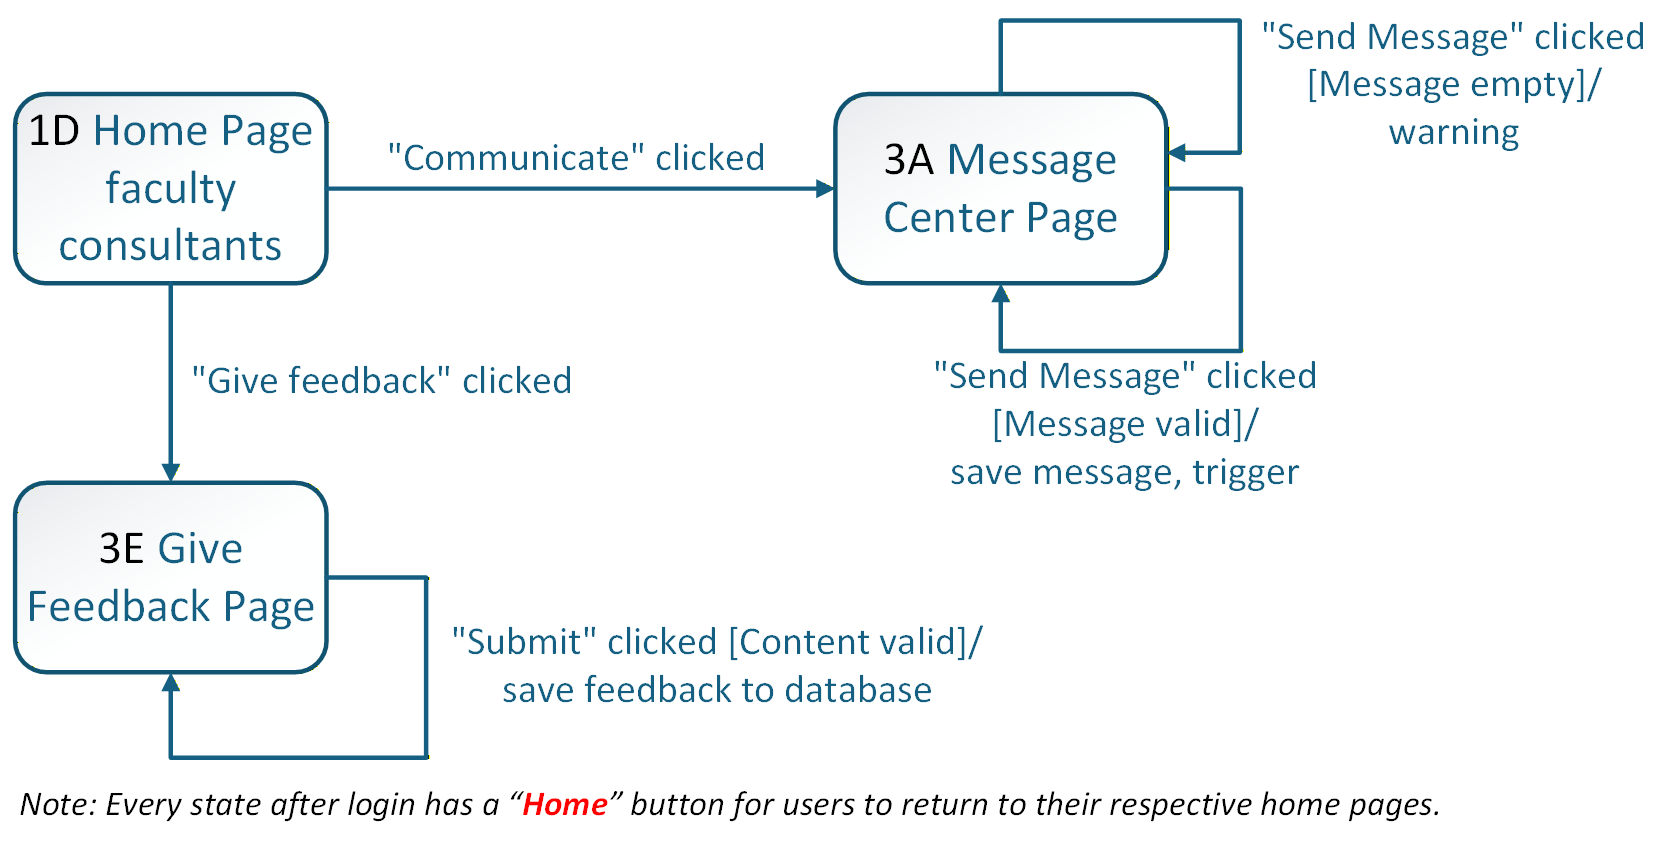
\includegraphics[width=\textwidth]{Page_5_docsmall.com.png}
\caption{Overview transition diagram for Communication and Give Feedback}
\label{fig:feedback-overview}
\end{figure}

\begin{figure}[H]
\centering
\includegraphics[width=\textwidth]{"Figure 2_5.pdf"}
\caption{Transition diagram for User Gives Feedback}
\label{fig:user-gives-feedback}
\end{figure}

\subsubsection{Stimulus/Response Sequences}

Scenario:

Actor: User (e.g., Mentor, Student, Coordinator, Faculty Consultant)

Assumption: The user has successfully logged into the system and is on the relevant Home Page.

Main Success Scenario:
\begin{enumerate}
\item The user clicks ``Give Feedback'' on the Home Page.
\item The system displays the 3E. Give Feedback Page.
\item The user enters feedback text.
\item The user clicks ``Submit''.
\item The system validates the input and saves the feedback.
\item The system displays a success confirmation and returns the user to the Home Page.
\end{enumerate}

Alternative Flows:

4a. If the user clicks ``Submit'' with empty content, the system displays an error message and remains on the 3E. Give Feedback Page.

4b. If the user clicks ``Cancel'' or ``Home'', the system discards any draft content and returns to the Home Page.

3a. If there are no feedback entries, the system displays an empty list message.

6a. If the reply fails due to a system error, the system displays an error message and allows retry.

\subsubsection{Functional Requirements}

REQ-1: The system shall provide a feedback submission interface for all logged-in user roles.

REQ-2: The system shall validate that feedback content is not empty before saving.

REQ-3: The system shall store the feedback together with user identity, role and submission time.

REQ-4: The system shall make submitted feedback available to Supporting Staff for later review.

%--------------------------------------------------------------
\subsection{View Log Info}

\subsubsection{Description and Priority}

This feature enables Supporting Staff to search and view system log information within a selected date range.

Priority: Medium

\begin{figure}[H]
\centering
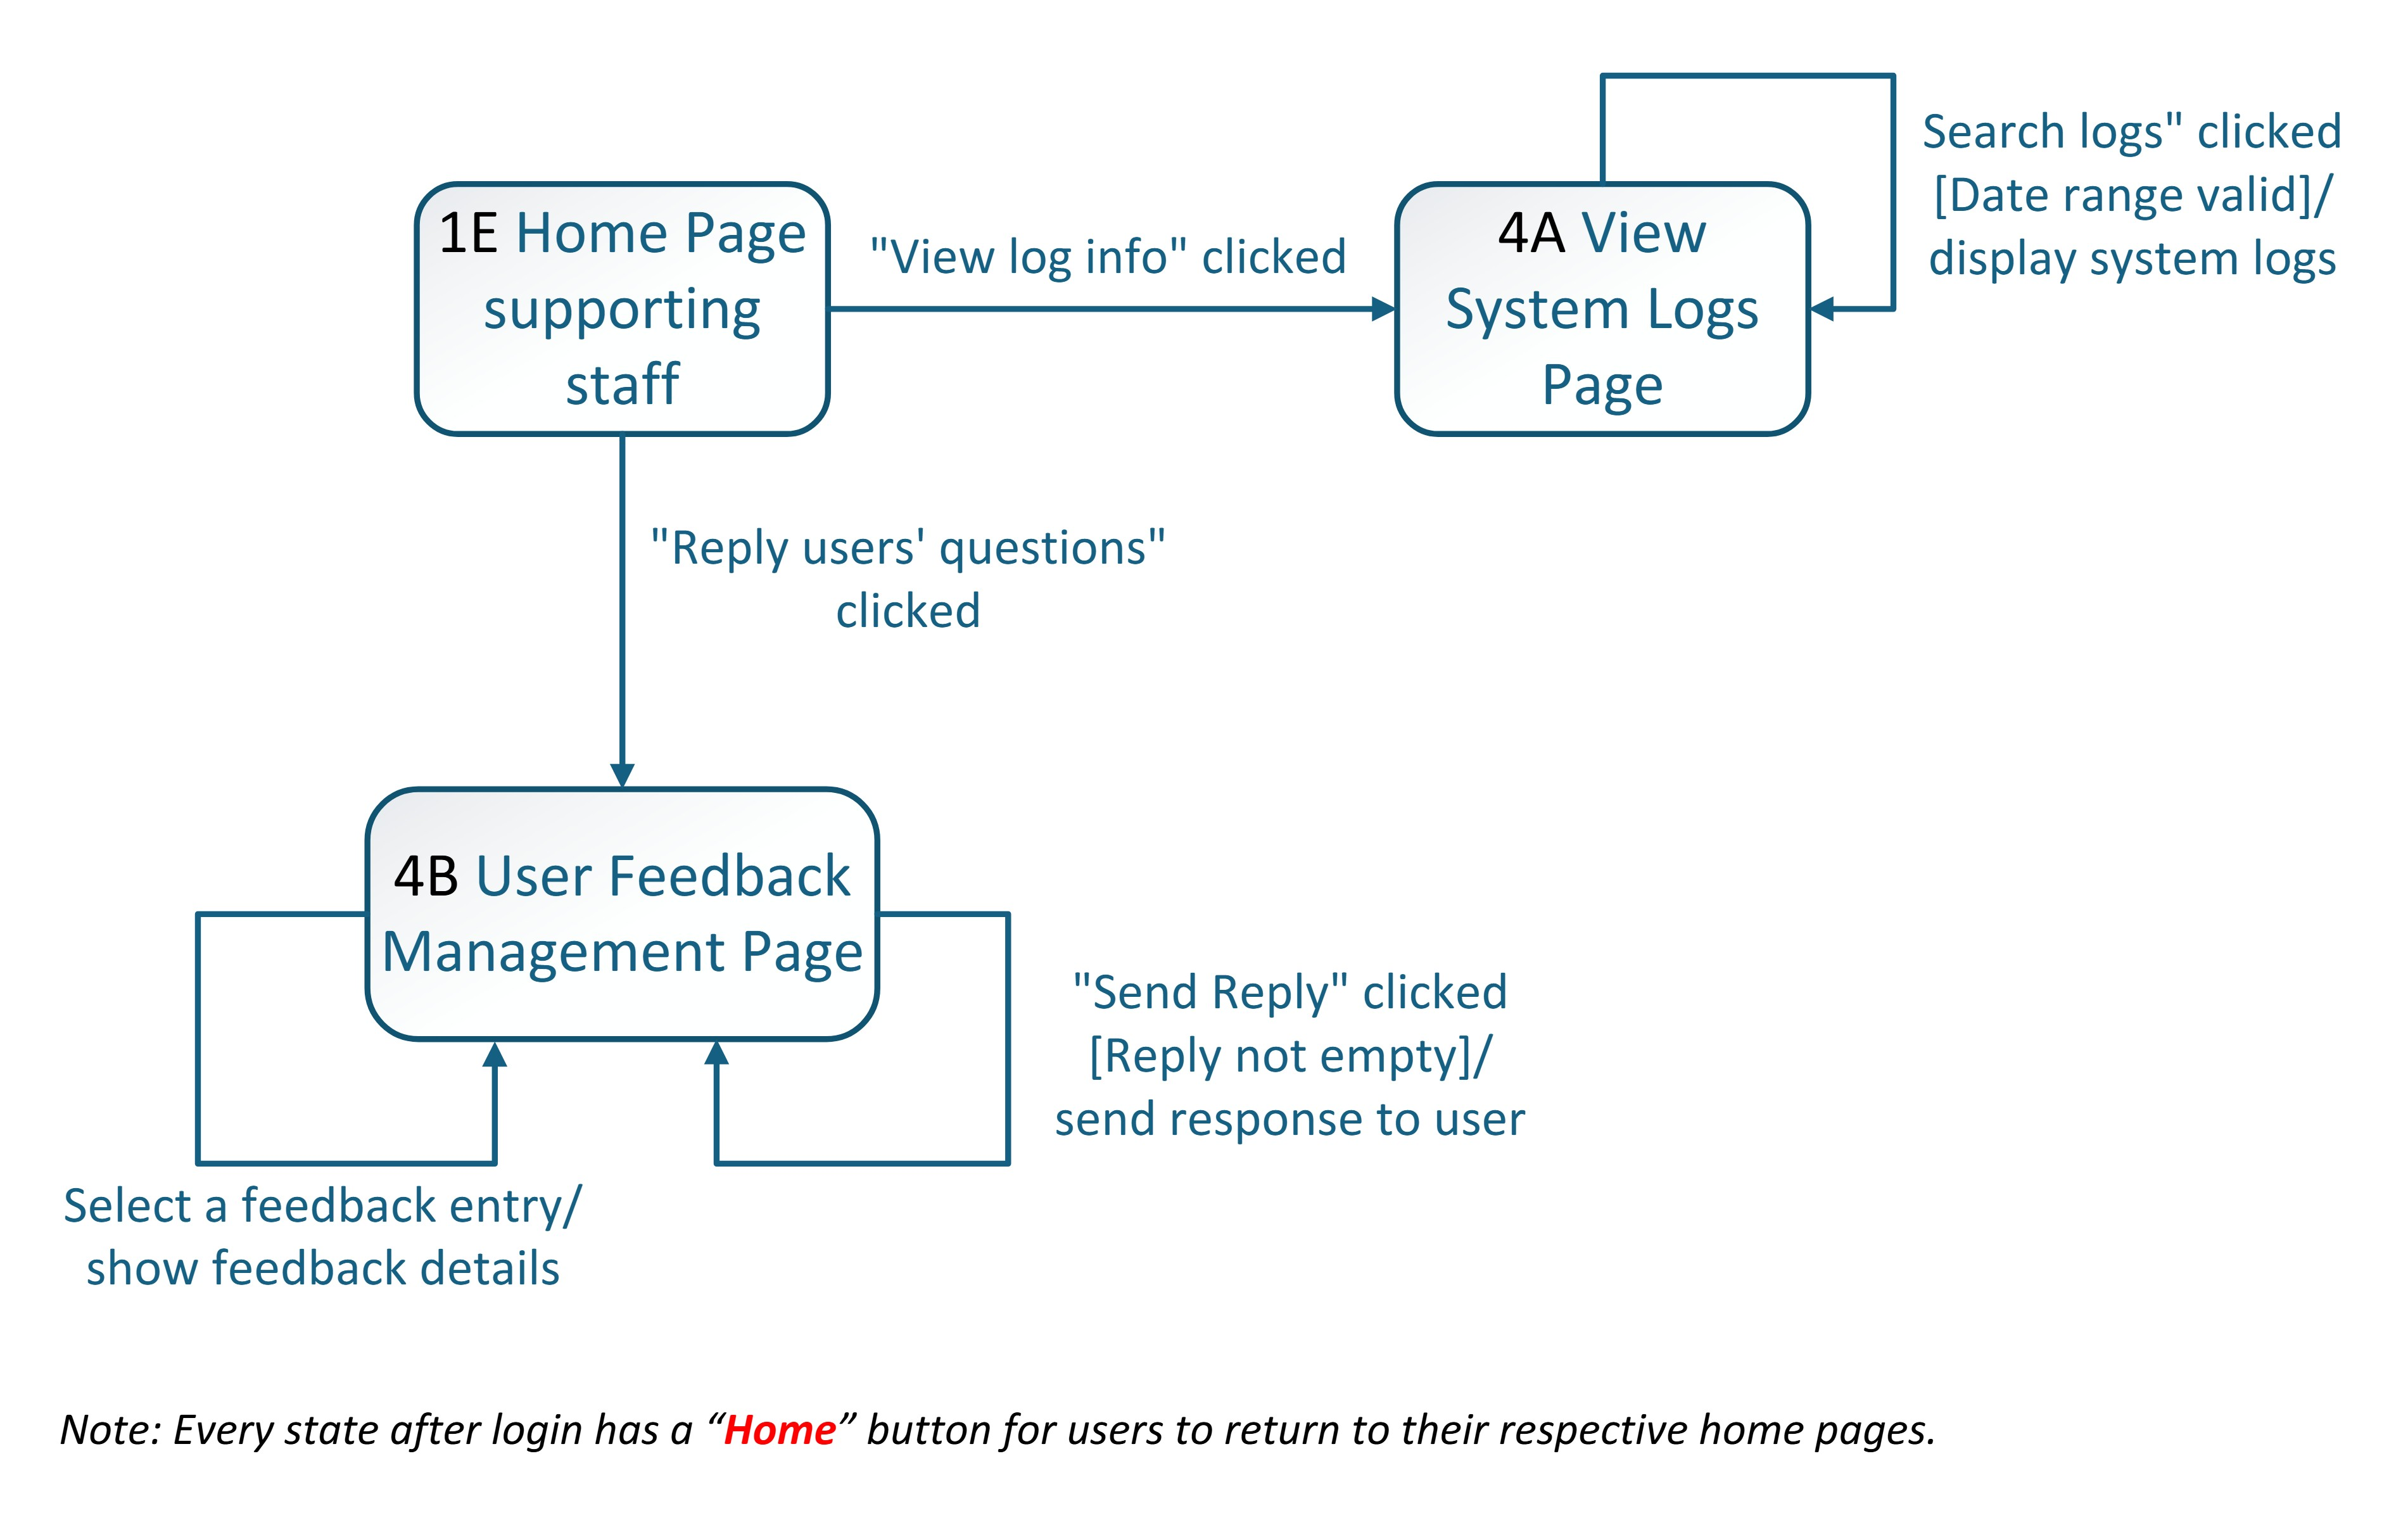
\includegraphics[width=\textwidth]{Page_6_docsmall.com.jpg}
\caption{Overview transition diagram for Supporting Staff functions}
\label{fig:view-log-overview}
\end{figure}

\subsubsection{Stimulus/Response Sequences}

Scenario 6: View Log Info

Actor: Supporting Staff

Assumption: The user has already logged into the system and is currently on the 1E. Home Page supporting staff.

Main Success Scenario:
\begin{enumerate}
\item User clicks the ``View log info'' button on the 1E. Home Page supporting staff.
\item System transitions to and displays the 4A. View System Logs Page.
\item User selects a valid Start Date and End Date, then clicks the ``Search logs'' button.
\item System retrieves the relevant login/logout times and core function usage logs and displays them in the list area.
\end{enumerate}

Alternative Flows:

3a. If the selected date range is invalid, the system displays a warning message and remains on the 4A. View System Logs Page.

4a. If no logs match the selected criteria, the system displays an empty result list with a corresponding notice.

\subsubsection{Functional Requirements}

REQ-1: The system shall allow Supporting Staff to search logs by date range.

REQ-2: The system shall display login/logout records and core function usage logs.

REQ-3: The system shall prevent unauthorized modification or deletion of log data through the viewing interface.

%--------------------------------------------------------------
\subsection{Reply to Users' Questions}

\subsubsection{Description and Priority}

This feature enables Supporting Staff to review feedback entries and reply to users' questions through the system.

Priority: Medium

\subsubsection{Stimulus/Response Sequences}

Transition diagram is included in 3.14.2.

Scenario 7: Reply to Users' Questions

Actor: Supporting Staff

Assumption: The user has already logged into the system and is currently on the 1E. Home Page supporting staff.

Main Success Scenario:
\begin{enumerate}
\item User clicks the ``Reply users' questions'' button on the 1E. Home Page supporting staff.
\item System transitions to and displays the 4B. Reply Feedback Page.
\item User selects a specific feedback entry from the Feedback List.
\item System displays the original user feedback text in the read-only display area.
\item User types a reply in the text editing area and clicks the ``Send Reply'' button.
\item System saves the response, updates the status of the feedback, and notifies the user who submitted the feedback.
\end{enumerate}

Alternative Flows:

5a. If the reply content is empty, the system displays a validation error and does not send the reply.

3a. If there are no feedback entries, the system displays an empty list message.

6a. If the reply fails due to a system error, the system displays an error message and allows retry.

\subsubsection{Functional Requirements}

REQ-1: The system shall allow Supporting Staff to access feedback entries submitted by users.

REQ-2: The system shall display the original feedback text in read-only form.

REQ-3: The system shall validate that reply content is not empty before sending.

REQ-4: The system shall save each reply together with responder identity and response time.

REQ-5: The system shall notify the user after a reply is successfully sent.

%--------------------------------------------------------------
\subsection{Set up Faculty Consultants}

\subsubsection{Description and Priority}

This feature enables the Administrator to add, modify or delete faculty consultants for each faculty in the system. The Administrator can search for staff members and assign them as faculty consultants for a specific faculty (FST, FHSS, FSM, DCC, or any newly added faculty).

Priority: High

\begin{figure}[H]
\centering
\includegraphics[width=\textwidth]{"Figure 2_6.pdf"}
\caption{Transition diagram for Set up Faculty Consultants}
\label{fig:setup-faculty-consultants}
\end{figure}

\subsubsection{Stimulus/Response Sequences}

Scenario:

Actor: Administrator

Assumption: The user has already logged into the system and is currently on the 4C. Admin Home Page.

Main Success Scenario:
\begin{enumerate}
\item The user clicks the ``Set up Faculty Consultants'' button on the 4C. Admin Home Page.
\item The system transitions to and displays the 4D. Set up Faculty Consultants Page, showing the current list of faculty consultants grouped by faculty.
\item The user selects a faculty from the dropdown and enters a Staff Name or ID in the search field, then clicks ``Search''.
\item The system retrieves and displays the staff member's basic information.
\item The user clicks the ``Save'' button.
\item The system assigns the staff member as the faculty consultant for the selected faculty, updates the database, and displays a success message.
\end{enumerate}

Alternative Flows:

3a. If the entered Staff Name or ID is invalid or not found, the system displays a warning message and remains on the 4D page.

5a. If the selected staff member is already assigned as a consultant for another faculty, the system displays a confirmation dialog before proceeding.

2a. The user clicks ``Edit'' or ``Delete'' next to an existing consultant entry to modify or remove the assignment.

\subsubsection{Functional Requirements}

REQ-1: The system shall allow only the Administrator to add, modify or delete faculty consultant assignments.

REQ-2: The system shall display the current list of faculty consultants grouped by faculty.

REQ-3: The system shall validate that the searched staff member exists in the BNBU school database.

REQ-4: The system shall record each faculty consultant assignment change in the system log.

REQ-5: The system shall support assigning one or more faculty consultants per faculty.

%--------------------------------------------------------------
\subsection{Set up Faculties and Departments}

\subsubsection{Description and Priority}

This feature enables the Administrator to configure the organizational architecture of BNBU, including faculties, departments and majors. The configuration can be done either manually through the system interface or by importing an Excel file (Appendix A format).

Priority: High

\begin{figure}[H]
\centering
\includegraphics[width=\textwidth]{"Figure 2_7.pdf"}
\caption{Transition diagram for Set up Faculties and Departments}
\label{fig:setup-faculties-departments}
\end{figure}

\subsubsection{Stimulus/Response Sequences}

Scenario:

Actor: Administrator

Assumption: The user has already logged into the system and is currently on the 4C. Admin Home Page.

Main Success Scenario (Manual Entry):
\begin{enumerate}
\item The user clicks the ``Set up Faculties and Departments'' button on the 4C. Admin Home Page.
\item The system transitions to and displays the 4E. Set up Faculties, Departments and Majors Page, showing the current organizational structure.
\item The user enters a Faculty Name, Department Name and Major Name in the respective input fields.
\item The user clicks the ``Save'' button.
\item The system validates the input and adds the new entry to the organizational structure, displaying a success message.
\end{enumerate}

Alternative Scenario (Excel Import):
\begin{enumerate}
\item The user clicks the ``Set up Faculties and Departments'' button on the 4C. Admin Home Page.
\item The system transitions to and displays the 4E. Set up Faculties, Departments and Majors Page.
\item The user clicks ``Upload Excel'' and selects a valid Excel file conforming to Appendix A format.
\item The system validates the file format and previews the uploaded data.
\item The user clicks ``Confirm Import''.
\item The system updates the organizational structure without overwriting existing data and displays a success message.
\end{enumerate}

Alternative Flows:

3a. If the user enters a Faculty/Department/Major name that already exists, the system displays a warning message.

3c. If the uploaded file is not in valid Excel format, the system displays a warning message and remains on the 4E page.

2a. The user clicks ``Edit'' or ``Delete'' next to an existing entry to modify or remove it.

\subsubsection{Functional Requirements}

REQ-1: The system shall allow only the Administrator to configure the organizational architecture.

REQ-2: The system shall support both manual entry and Excel file import (Appendix A format) for configuring faculties, departments and majors.

REQ-3: The system shall display the current organizational structure in a viewable format.

REQ-4: The system shall validate that no duplicate entries are created.

REQ-5: The system shall support the dynamic addition of new faculties without modifying the core system code.

REQ-6: The system shall not overwrite existing organizational data when importing from Excel; only non-existing information is updated.

REQ-7: The system shall record each organizational structure change in the system log.

%--------------------------------------------------------------
\subsection{Set up Supporting Staff}

\subsubsection{Description and Priority}

This feature enables the Administrator to search for a staff member in the BNBU school database and assign the Supporting Staff role to that person.

Priority: High

\begin{figure}[H]
\centering
\includegraphics[width=\textwidth]{"Figure 2_8.pdf"}
\caption{Transition diagram for Set up Supporting Staff}
\label{fig:setup-supporting-staff}
\end{figure}

\subsubsection{Stimulus/Response Sequences}

Scenario:

Actor: Administrator

Assumption: The user has already logged into the system and is currently on the 4C. Admin Home Page.

Main Success Scenario:
\begin{enumerate}
\item The user clicks the ``Set up Supporting Staff'' button on the 4C. Admin Home Page.
\item The system transitions to and displays the 4F. Set up Supporting Staff Page, showing the current supporting staff member (if any).
\item The user enters a Staff ID or Name in the search field and clicks ``Search''.
\item The system retrieves and displays the staff member's basic information from the BNBU school database.
\item The user clicks the ``Assign as Supporting Staff'' button.
\item The system updates the staff member's role to Supporting Staff in the database and displays a success message.
\end{enumerate}

Alternative Flows:

3a. If the entered Staff ID or Name is invalid or not found in the school database, the system displays a warning message.

5a. If a Supporting Staff member is already assigned, the system asks for confirmation before replacing.

2a. The user clicks ``Remove'' next to the current supporting staff entry to revoke the role assignment.

\subsubsection{Functional Requirements}

REQ-1: The system shall allow only the Administrator to assign or remove the Supporting Staff role.

REQ-2: The system shall search for staff members from the BNBU school database by Staff ID or Name.

REQ-3: The system shall display the current supporting staff assignment.

REQ-4: The system shall update the staff member's role permissions after a valid assignment.

REQ-5: The system shall record each supporting staff assignment change in the system log.


% 4. External Interface Requirements
%--------------------------------------------------------------
% Section 4: External Interface Requirements
\section{External Interface Requirements}

\subsection{User Interfaces}

Please refer to the separate document named `B04 Section3 UI\_Diagrams.pdf' for all user interface designs corresponding to the state transition diagrams.

\subsection{Hardware Interfaces}

The Mentor Caring System primarily operates on standard computing equipment and does not require any specialized hardware devices.

Users shall interact with the system through ordinary personal computers or laptops using common input and output devices such as keyboards, mice, and displays.

On the server side, the system shall be hosted on standard server hardware that supports the execution of the web application, storage of system data, and communication with external university services. The system shall also rely on normal network infrastructure to enable communication between client devices, the MCS server, the BNBU school database, and the BNBU email service.

The system does not directly control or manipulate external hardware devices. All hardware interaction shall be limited to ordinary web-based input, display, storage, and network communication functions. This is aligned with the project description, which presents MCS as a supporting management system rather than a hardware control system.

\subsection{Software Interfaces}

The Mentor Caring System interacts with several external software components that support its operation:

\textbf{BNBU School Database System:} Provides user authentication information including account ID, password, user name and role type. The MCS accesses this database in read-only mode for login verification.

\textbf{Relational Database Management System:} The system stores its operational data (mentor allocation, interview records, communication messages and logs) in a dedicated database such as MySQL 8.0 or Microsoft SQL Server 2019.

\textbf{Web Server Software:} Application deployment is supported by web servers such as Nginx or Apache Tomcat, which manage HTTP requests, session management and application service execution.

\textbf{Email Server System:} The BNBU email server is used to send automatic notification emails whenever a system message or interview appointment is created.

\textbf{Office Software Integration:} Microsoft Excel is used for importing structured data such as student lists and mentor allocations, while Microsoft Word is used for exporting reports and interview records.

\subsection{Communications Interfaces}

The Mentor Caring System relies on standard network communication technologies to support user access and system messaging:

\textbf{Web Communication:} Users shall access the system interfaces through a standard secure web network connection (such as HTTPS).

\textbf{Email Notification Service:} The system shall communicate with the BNBU email service using standard mail transport protocols to automatically send notifications to the receiving parties.

\textbf{Network Access:} Internal users can access the system via the BNBU campus network, while external access shall rely on the university's existing secure network access arrangements (such as a campus VPN).

%--------------------------------------------------------------
% 5. Other Nonfunctional Requirements
%--------------------------------------------------------------
% Section 5: Other Nonfunctional Requirements
\section{Other Nonfunctional Requirements}

\subsection{Performance Requirements}

The Mentor Caring System must meet the following measurable performance requirements:

\textbf{System Response Time:}

The system shall return results for common user operations (including login verification, student/mentor information search, and message viewing) within 2 seconds under normal network conditions ($\leq$200 ms latency, stable campus network).

\textbf{Concurrent Users:}

The system shall support at least 300 concurrent users during peak usage periods (e.g., mentor allocation period at the beginning of the academic year) without performance degradation (i.e., response time shall not exceed 3 seconds for 95\% of requests).

\textbf{File Import/Export Performance:}

The system shall complete batch Excel file import (up to 1000 records per file) within 5 seconds, and generate/export Word reports (up to 100 pages) within 10 seconds under normal system load.

\textbf{System Availability:}

The system shall achieve at least 99\% uptime during normal academic operation periods (excluding scheduled maintenance), and any single system downtime shall not exceed 30 minutes.

\subsection{Safety Requirements}

No specific safety requirements are defined for the Mentor Caring System, as the system does not involve any hardware control or safety-critical operations.

\subsection{Security Requirements}

Security is critical for protecting sensitive academic and personal information stored in the Mentor Caring System.

\textbf{User Authentication:} All users must log in using their BNBU university accounts verified through the school database.

\textbf{Role-Based Access Control:} Access to system functions must be strictly controlled according to user roles (administrator, faculty consultant, mentor, student, MCP coordinator, supporting staff).

\textbf{Data Privacy Protection:} Student personal information, interview records and communication messages must only be accessible to authorized users.

\textbf{Secure Communication:} All login sessions and sensitive data transfers must use encrypted HTTPS connections.

\textbf{Log Monitoring:} The system must record login and logout times and major user actions for auditing and security monitoring purposes.

\subsection{Software Quality Attributes}

The Mentor Caring System must satisfy several important software quality attributes:

\textbf{Usability:} The web interface should be intuitive and easy to use so that users with basic computer skills can operate the system without extensive training.

\textbf{Reliability:} The system should operate continuously with minimal failures and should recover gracefully from unexpected errors.

\textbf{Maintainability:} The system architecture should follow modular design principles and include clear documentation and code comments to facilitate future maintenance.

\textbf{Scalability:} The system should allow the addition of new faculties, departments and users without major structural modifications.

\textbf{Portability:} The web-based architecture ensures that the system can run on multiple operating systems and browsers.

\textbf{Testability:} Functional modules should be designed so that they can be independently tested during development and quality assurance.

%--------------------------------------------------------------
% 6. Other Requirements
%--------------------------------------------------------------
% Section 6: Other Requirements
\section{Other Requirements}

\textbf{Database Requirements:} The system must maintain an independent database storing mentor groups, student information, interview records, communication messages and system logs.

\textbf{Data Retention Policy:} Historical records of mentor allocations and interview reports must be permanently retained for management and auditing purposes.

\textbf{Legal and Policy Compliance:} The system must comply with BNBU information management policies and relevant regulations on data protection and privacy.

\textbf{Future Expansion Considerations:} The system design should allow future integration with other BNBU information systems such as student management platforms or learning management systems.

%--------------------------------------------------------------
% Appendices
% Appendices
\appendix

\section*{Appendix A: Glossary}
\addcontentsline{toc}{section}{Appendix A: Glossary}

\section*{Appendix B: Analysis Models}
\addcontentsline{toc}{section}{Appendix B: Analysis Models}

\subsection*{B.1 Sequence Diagram}
\begin{figure}[H]
    \centering
    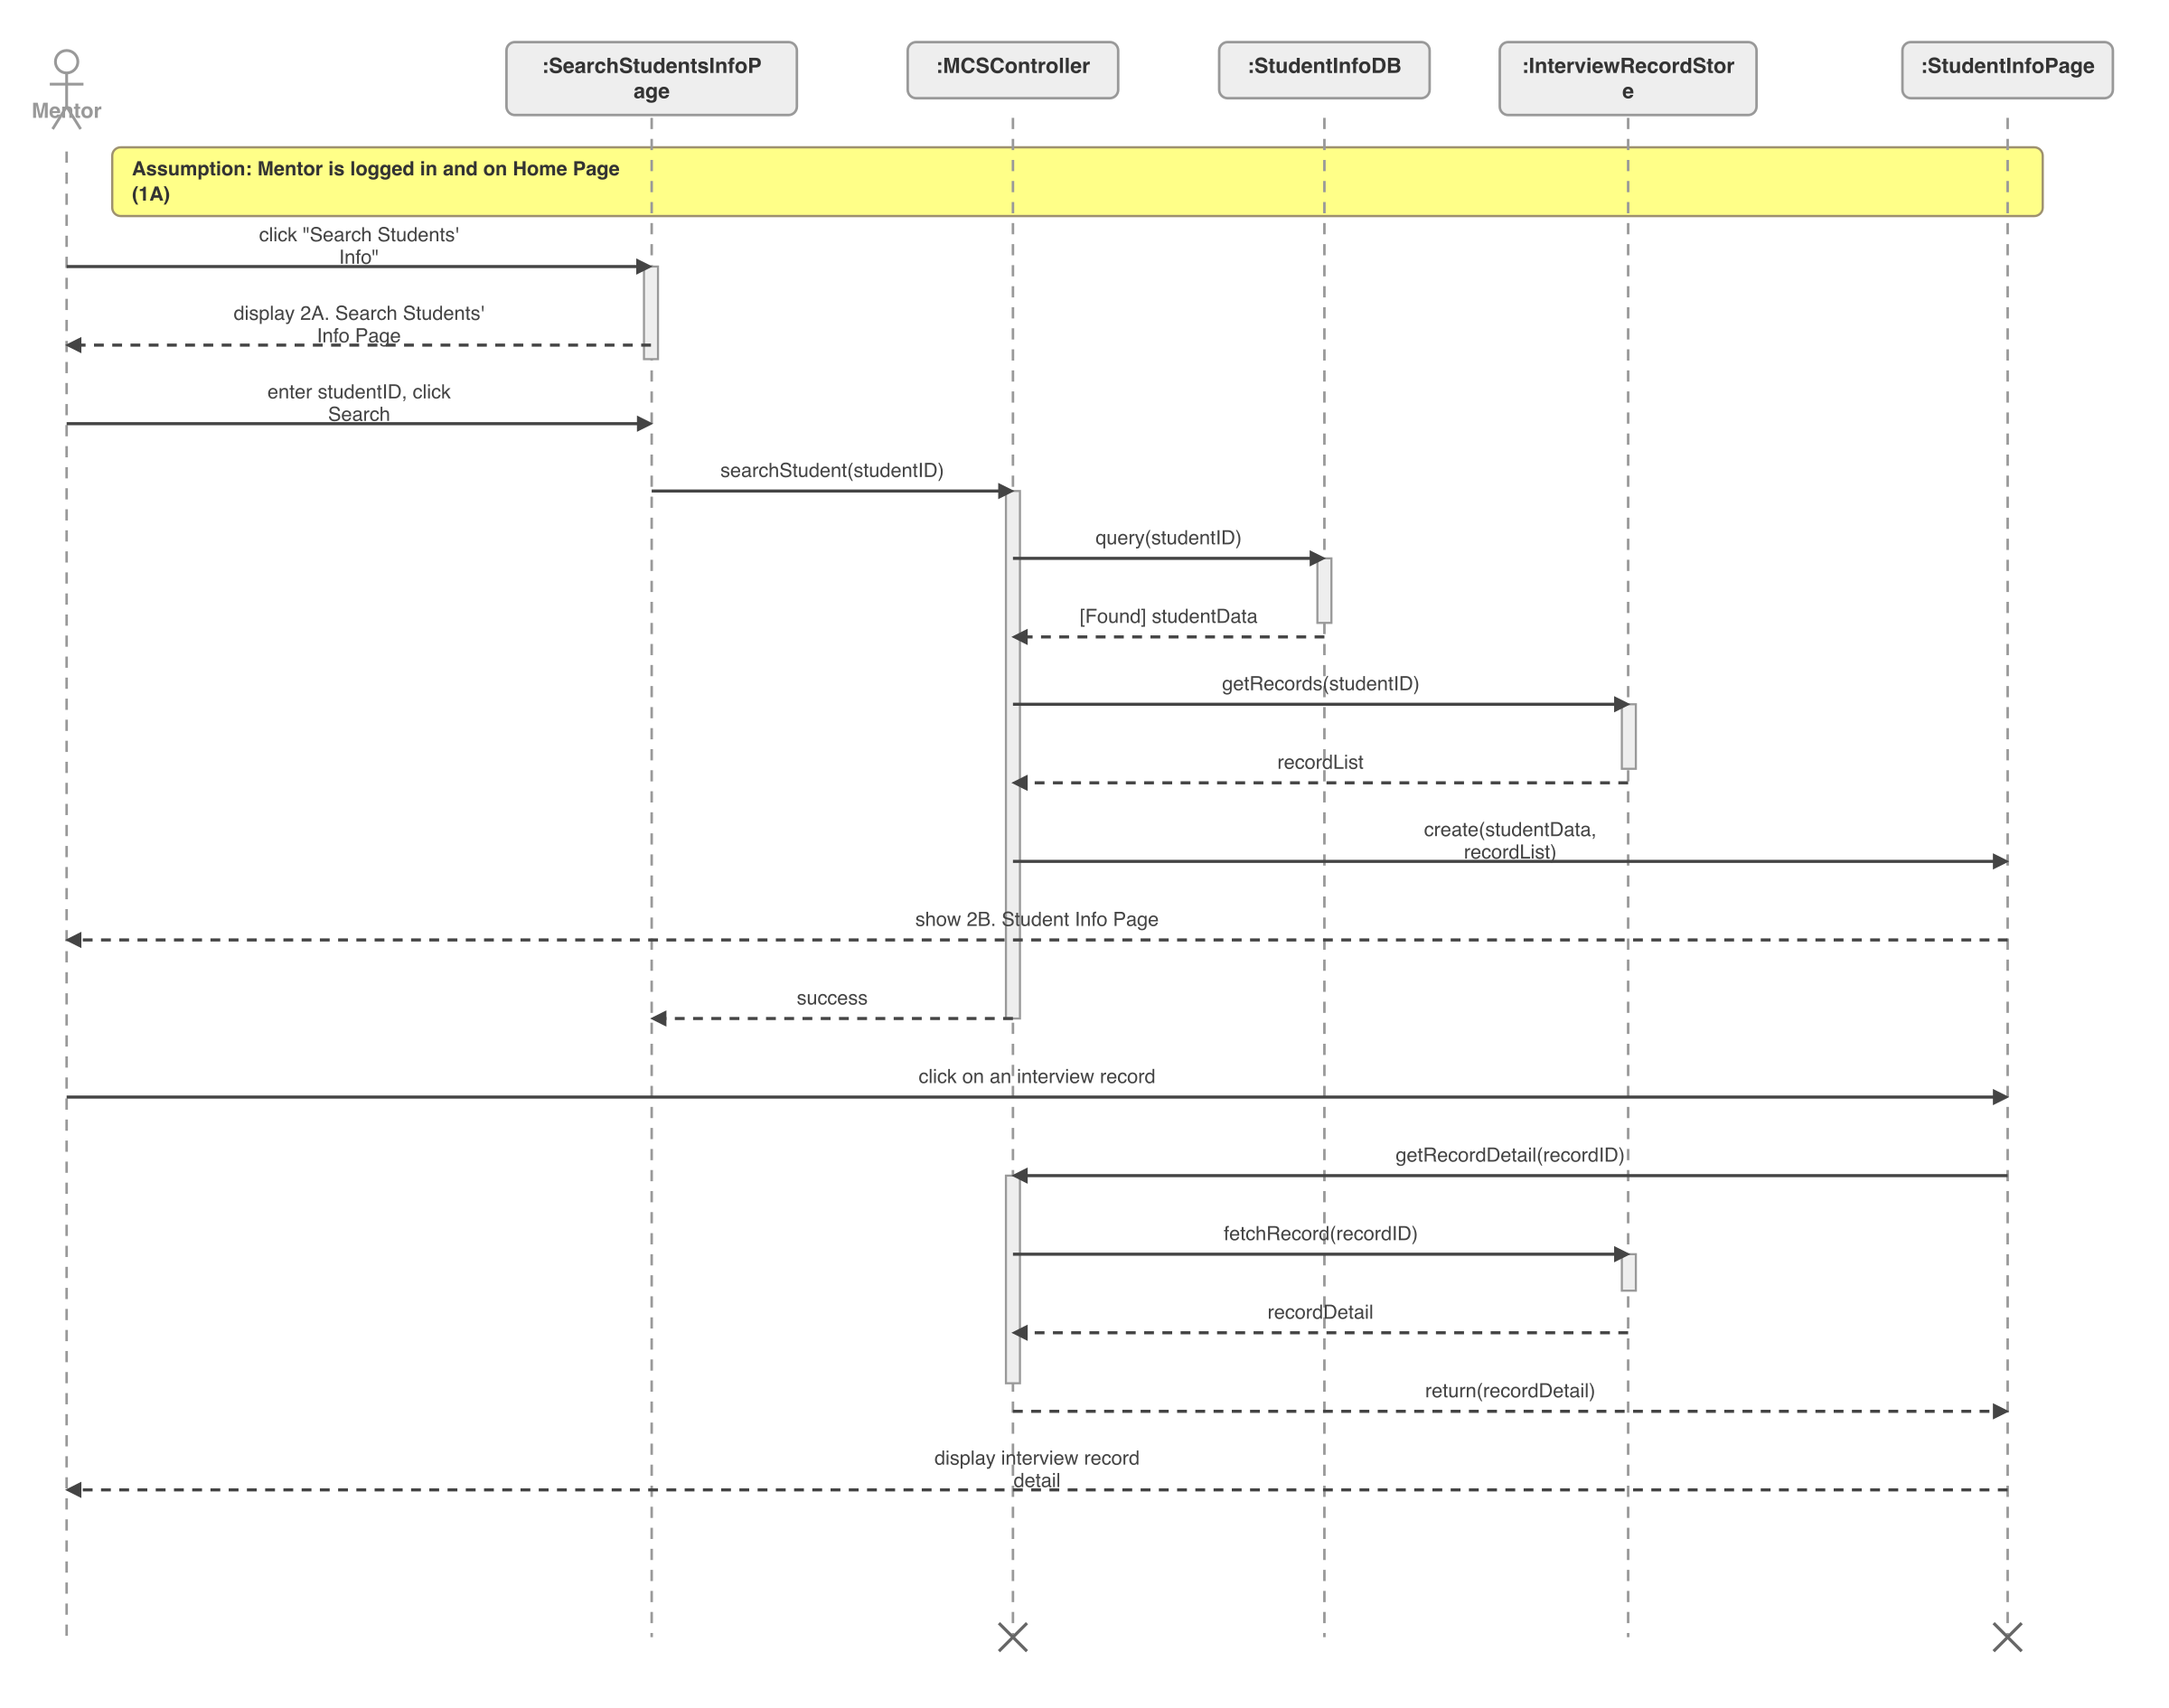
\includegraphics[width=\textwidth,height=0.82\textheight,keepaspectratio]{seq.png}
    \caption{Sequence Diagram}
    \label{fig:seq_diagram}
\end{figure}

\clearpage

\subsection*{B.2 Class Diagram}
\begin{figure}[H]
    \centering
    \includegraphics[width=\textwidth,height=0.84\textheight,keepaspectratio]{"Lab 6 Class Diagram.png"}
    \caption{Class Diagram}
    \label{fig:class_diagram}
\end{figure}

\section*{Appendix C: Issues List}
\addcontentsline{toc}{section}{Appendix C: Issues List}

\end{document}
